\documentclass[twoside]{book}

% Packages required by doxygen
\usepackage{fixltx2e}
\usepackage{calc}
\usepackage{doxygen}
\usepackage[export]{adjustbox} % also loads graphicx
\usepackage{graphicx}
\usepackage[utf8]{inputenc}
\usepackage{makeidx}
\usepackage{multicol}
\usepackage{multirow}
\PassOptionsToPackage{warn}{textcomp}
\usepackage{textcomp}
\usepackage[nointegrals]{wasysym}
\usepackage[table]{xcolor}

% Font selection
\usepackage[T1]{fontenc}
\usepackage[scaled=.90]{helvet}
\usepackage{courier}
\usepackage{amssymb}
\usepackage{sectsty}
\renewcommand{\familydefault}{\sfdefault}
\allsectionsfont{%
  \fontseries{bc}\selectfont%
  \color{darkgray}%
}
\renewcommand{\DoxyLabelFont}{%
  \fontseries{bc}\selectfont%
  \color{darkgray}%
}
\newcommand{\+}{\discretionary{\mbox{\scriptsize$\hookleftarrow$}}{}{}}

% Page & text layout
\usepackage{geometry}
\geometry{%
  a4paper,%
  top=2.5cm,%
  bottom=2.5cm,%
  left=2.5cm,%
  right=2.5cm%
}
\tolerance=750
\hfuzz=15pt
\hbadness=750
\setlength{\emergencystretch}{15pt}
\setlength{\parindent}{0cm}
\setlength{\parskip}{3ex plus 2ex minus 2ex}
\makeatletter
\renewcommand{\paragraph}{%
  \@startsection{paragraph}{4}{0ex}{-1.0ex}{1.0ex}{%
    \normalfont\normalsize\bfseries\SS@parafont%
  }%
}
\renewcommand{\subparagraph}{%
  \@startsection{subparagraph}{5}{0ex}{-1.0ex}{1.0ex}{%
    \normalfont\normalsize\bfseries\SS@subparafont%
  }%
}
\makeatother

% Headers & footers
\usepackage{fancyhdr}
\pagestyle{fancyplain}
\fancyhead[LE]{\fancyplain{}{\bfseries\thepage}}
\fancyhead[CE]{\fancyplain{}{}}
\fancyhead[RE]{\fancyplain{}{\bfseries\leftmark}}
\fancyhead[LO]{\fancyplain{}{\bfseries\rightmark}}
\fancyhead[CO]{\fancyplain{}{}}
\fancyhead[RO]{\fancyplain{}{\bfseries\thepage}}
\fancyfoot[LE]{\fancyplain{}{}}
\fancyfoot[CE]{\fancyplain{}{}}
\fancyfoot[RE]{\fancyplain{}{\bfseries\scriptsize Generated by Doxygen }}
\fancyfoot[LO]{\fancyplain{}{\bfseries\scriptsize Generated by Doxygen }}
\fancyfoot[CO]{\fancyplain{}{}}
\fancyfoot[RO]{\fancyplain{}{}}
\renewcommand{\footrulewidth}{0.4pt}
\renewcommand{\chaptermark}[1]{%
  \markboth{#1}{}%
}
\renewcommand{\sectionmark}[1]{%
  \markright{\thesection\ #1}%
}

% Indices & bibliography
\usepackage{natbib}
\usepackage[titles]{tocloft}
\setcounter{tocdepth}{3}
\setcounter{secnumdepth}{5}
\makeindex

% Hyperlinks (required, but should be loaded last)
\usepackage{ifpdf}
\ifpdf
  \usepackage[pdftex,pagebackref=true]{hyperref}
\else
  \usepackage[ps2pdf,pagebackref=true]{hyperref}
\fi
\hypersetup{%
  colorlinks=true,%
  linkcolor=blue,%
  citecolor=blue,%
  unicode%
}

% Custom commands
\newcommand{\clearemptydoublepage}{%
  \newpage{\pagestyle{empty}\cleardoublepage}%
}

\usepackage{caption}
\captionsetup{labelsep=space,justification=centering,font={bf},singlelinecheck=off,skip=4pt,position=top}

%===== C O N T E N T S =====

\begin{document}

% Titlepage & ToC
\hypersetup{pageanchor=false,
             bookmarksnumbered=true,
             pdfencoding=unicode
            }
\pagenumbering{alph}
\begin{titlepage}
\vspace*{7cm}
\begin{center}%
{\Large My Project }\\
\vspace*{1cm}
{\large Generated by Doxygen 1.8.14}\\
\end{center}
\end{titlepage}
\clearemptydoublepage
\pagenumbering{roman}
\tableofcontents
\clearemptydoublepage
\pagenumbering{arabic}
\hypersetup{pageanchor=true}

%--- Begin generated contents ---
\chapter{Hierarchical Index}
\section{Class Hierarchy}
This inheritance list is sorted roughly, but not completely, alphabetically\+:\begin{DoxyCompactList}
\item \contentsline{section}{Button\+Listener}{\pageref{class_button_listener}}{}
\begin{DoxyCompactList}
\item \contentsline{section}{Shoot\+Control}{\pageref{class_shoot_control}}{}
\end{DoxyCompactList}
\item \contentsline{section}{ir\+\_\+msg}{\pageref{structir__msg}}{}
\item \contentsline{section}{I\+R\+Control}{\pageref{class_i_r_control}}{}
\begin{DoxyCompactList}
\item \contentsline{section}{Shoot\+Control}{\pageref{class_shoot_control}}{}
\end{DoxyCompactList}
\item \contentsline{section}{msg\+\_\+listener}{\pageref{classmsg__listener}}{}
\begin{DoxyCompactList}
\item \contentsline{section}{msg\+\_\+logger}{\pageref{classmsg__logger}}{}
\end{DoxyCompactList}
\item \contentsline{section}{pause\+\_\+listener}{\pageref{classpause__listener}}{}
\begin{DoxyCompactList}
\item \contentsline{section}{msg\+\_\+decoder}{\pageref{classmsg__decoder}}{}
\end{DoxyCompactList}
\item task\begin{DoxyCompactList}
\item \contentsline{section}{Button}{\pageref{class_button}}{}
\item \contentsline{section}{msg\+\_\+decoder}{\pageref{classmsg__decoder}}{}
\item \contentsline{section}{msg\+\_\+logger}{\pageref{classmsg__logger}}{}
\item \contentsline{section}{pause\+\_\+detector}{\pageref{classpause__detector}}{}
\item \contentsline{section}{Shoot\+Control}{\pageref{class_shoot_control}}{}
\end{DoxyCompactList}
\end{DoxyCompactList}

\chapter{Class Index}
\section{Class List}
Here are the classes, structs, unions and interfaces with brief descriptions\+:\begin{DoxyCompactList}
\item\contentsline{section}{\mbox{\hyperlink{class_button}{Button}} \\*This class is used to make a button object }{\pageref{class_button}}{}
\item\contentsline{section}{\mbox{\hyperlink{class_button_listener}{Button\+Listener}} \\*A class containing the virtual button\+Pressed function }{\pageref{class_button_listener}}{}
\item\contentsline{section}{\mbox{\hyperlink{class_buzzer_control}{Buzzer\+Control}} \\*This class is used to control the buzzer }{\pageref{class_buzzer_control}}{}
\item\contentsline{section}{\mbox{\hyperlink{class_display_control}{Display\+Control}} \\*This class is used to show the command value on the screen }{\pageref{class_display_control}}{}
\item\contentsline{section}{\mbox{\hyperlink{class_game_leader}{Game\+Leader}} \\*This class is used to make the game }{\pageref{class_game_leader}}{}
\item\contentsline{section}{\mbox{\hyperlink{class_game_logs}{Game\+Logs}} \\*This class is used to track all the hits during the game and to print them at the end }{\pageref{class_game_logs}}{}
\item\contentsline{section}{\mbox{\hyperlink{structir__msg}{ir\+\_\+msg}} \\*This struct gets used to split the message in two parts }{\pageref{structir__msg}}{}
\item\contentsline{section}{\mbox{\hyperlink{class_i_r_control}{I\+R\+Control}} \\*This class is used to control the IR signal }{\pageref{class_i_r_control}}{}
\item\contentsline{section}{\mbox{\hyperlink{class_keypad}{Keypad}} \\*In this class you can find the pin setup and initialize the characters }{\pageref{class_keypad}}{}
\item\contentsline{section}{\mbox{\hyperlink{class_keypad_control}{Keypad\+Control}} \\*This class is used to control the keypad }{\pageref{class_keypad_control}}{}
\item\contentsline{section}{\mbox{\hyperlink{classmsg__decoder}{msg\+\_\+decoder}} }{\pageref{classmsg__decoder}}{}
\item\contentsline{section}{\mbox{\hyperlink{classmsg__listener}{msg\+\_\+listener}} }{\pageref{classmsg__listener}}{}
\item\contentsline{section}{\mbox{\hyperlink{classmsg__logger}{msg\+\_\+logger}} }{\pageref{classmsg__logger}}{}
\item\contentsline{section}{\mbox{\hyperlink{class_msg_decoder}{Msg\+Decoder}} \\*This class decodes the incoming message and sends it to another class }{\pageref{class_msg_decoder}}{}
\item\contentsline{section}{\mbox{\hyperlink{class_msg_listener}{Msg\+Listener}} \\*This class constains the virtual msg\+Received function }{\pageref{class_msg_listener}}{}
\item\contentsline{section}{\mbox{\hyperlink{classpause__detector}{pause\+\_\+detector}} }{\pageref{classpause__detector}}{}
\item\contentsline{section}{\mbox{\hyperlink{classpause__listener}{pause\+\_\+listener}} }{\pageref{classpause__listener}}{}
\item\contentsline{section}{\mbox{\hyperlink{class_pause_detector}{Pause\+Detector}} \\*This class detects the pauses in a IR signal and sends them to another class }{\pageref{class_pause_detector}}{}
\item\contentsline{section}{\mbox{\hyperlink{class_pause_listener}{Pause\+Listener}} \\*This class contains the virtual function pause\+Detected }{\pageref{class_pause_listener}}{}
\item\contentsline{section}{\mbox{\hyperlink{class_player_control}{Player\+Control}} \\*This class controls the player tasks }{\pageref{class_player_control}}{}
\item\contentsline{section}{\mbox{\hyperlink{class_player_data}{Player\+Data}} \\*This class contains all the playerdata }{\pageref{class_player_data}}{}
\item\contentsline{section}{\mbox{\hyperlink{class_send_control}{Send\+Control}} \\*This class is used to send the data }{\pageref{class_send_control}}{}
\item\contentsline{section}{\mbox{\hyperlink{class_shoot_control}{Shoot\+Control}} \\*This class encodes and sends the message to be sent to the \mbox{\hyperlink{class_i_r_control}{I\+R\+Control}} class and controls the laser }{\pageref{class_shoot_control}}{}
\item\contentsline{section}{\mbox{\hyperlink{class_weapon}{Weapon}} \\*This class contains the data of the weapon }{\pageref{class_weapon}}{}
\end{DoxyCompactList}

\chapter{File Index}
\section{File List}
Here is a list of all documented files with brief descriptions\+:\begin{DoxyCompactList}
\item\contentsline{section}{C\+:/ti-\/software/thema\+\_\+opdracht\+\_\+lasergame/\+Player/\mbox{\hyperlink{_button_8hpp}{Button.\+hpp}} }{\pageref{_button_8hpp}}{}
\item\contentsline{section}{C\+:/ti-\/software/thema\+\_\+opdracht\+\_\+lasergame/\+Player/\mbox{\hyperlink{_button_listener_8hpp}{Button\+Listener.\+hpp}} }{\pageref{_button_listener_8hpp}}{}
\item\contentsline{section}{C\+:/ti-\/software/thema\+\_\+opdracht\+\_\+lasergame/\+Player/\mbox{\hyperlink{_buzzer_control_8hpp}{Buzzer\+Control.\+hpp}} }{\pageref{_buzzer_control_8hpp}}{}
\item\contentsline{section}{C\+:/ti-\/software/thema\+\_\+opdracht\+\_\+lasergame/\+Player/\mbox{\hyperlink{_display_control_8hpp}{Display\+Control.\+hpp}} }{\pageref{_display_control_8hpp}}{}
\item\contentsline{section}{C\+:/ti-\/software/thema\+\_\+opdracht\+\_\+lasergame/\+Player/\mbox{\hyperlink{_game_logs_8hpp}{Game\+Logs.\+hpp}} }{\pageref{_game_logs_8hpp}}{}
\item\contentsline{section}{C\+:/ti-\/software/thema\+\_\+opdracht\+\_\+lasergame/\+Player/\mbox{\hyperlink{_i_r_control_8hpp}{I\+R\+Control.\+hpp}} }{\pageref{_i_r_control_8hpp}}{}
\item\contentsline{section}{C\+:/ti-\/software/thema\+\_\+opdracht\+\_\+lasergame/\+Player/\mbox{\hyperlink{_keypad_8hpp}{Keypad.\+hpp}} }{\pageref{_keypad_8hpp}}{}
\item\contentsline{section}{C\+:/ti-\/software/thema\+\_\+opdracht\+\_\+lasergame/\+Player/\mbox{\hyperlink{_keypad_control_8hpp}{Keypad\+Control.\+hpp}} }{\pageref{_keypad_control_8hpp}}{}
\item\contentsline{section}{C\+:/ti-\/software/thema\+\_\+opdracht\+\_\+lasergame/\+Player/\mbox{\hyperlink{_msg_decoder_8hpp}{Msg\+Decoder.\+hpp}} }{\pageref{_msg_decoder_8hpp}}{}
\item\contentsline{section}{C\+:/ti-\/software/thema\+\_\+opdracht\+\_\+lasergame/\+Player/\mbox{\hyperlink{_msg_listener_8hpp}{Msg\+Listener.\+hpp}} }{\pageref{_msg_listener_8hpp}}{}
\item\contentsline{section}{C\+:/ti-\/software/thema\+\_\+opdracht\+\_\+lasergame/\+Player/\mbox{\hyperlink{_pause_detector_8hpp}{Pause\+Detector.\+hpp}} }{\pageref{_pause_detector_8hpp}}{}
\item\contentsline{section}{C\+:/ti-\/software/thema\+\_\+opdracht\+\_\+lasergame/\+Player/\mbox{\hyperlink{_pause_listener_8hpp}{Pause\+Listener.\+hpp}} }{\pageref{_pause_listener_8hpp}}{}
\item\contentsline{section}{C\+:/ti-\/software/thema\+\_\+opdracht\+\_\+lasergame/\+Player/\mbox{\hyperlink{_player_control_8hpp}{Player\+Control.\+hpp}} }{\pageref{_player_control_8hpp}}{}
\item\contentsline{section}{C\+:/ti-\/software/thema\+\_\+opdracht\+\_\+lasergame/\+Player/\mbox{\hyperlink{_player_data_8hpp}{Player\+Data.\+hpp}} }{\pageref{_player_data_8hpp}}{}
\item\contentsline{section}{C\+:/ti-\/software/thema\+\_\+opdracht\+\_\+lasergame/\+Player/\mbox{\hyperlink{_shoot_control_8hpp}{Shoot\+Control.\+hpp}} }{\pageref{_shoot_control_8hpp}}{}
\item\contentsline{section}{C\+:/ti-\/software/thema\+\_\+opdracht\+\_\+lasergame/\+Player/\mbox{\hyperlink{_weapon_8hpp}{Weapon.\+hpp}} }{\pageref{_weapon_8hpp}}{}
\end{DoxyCompactList}

\chapter{Class Documentation}
\hypertarget{class_button}{}\section{Button Class Reference}
\label{class_button}\index{Button@{Button}}


This class is used to make a button object.  




{\ttfamily \#include $<$Button.\+hpp$>$}

Inheritance diagram for Button\+:\begin{figure}[H]
\begin{center}
\leavevmode
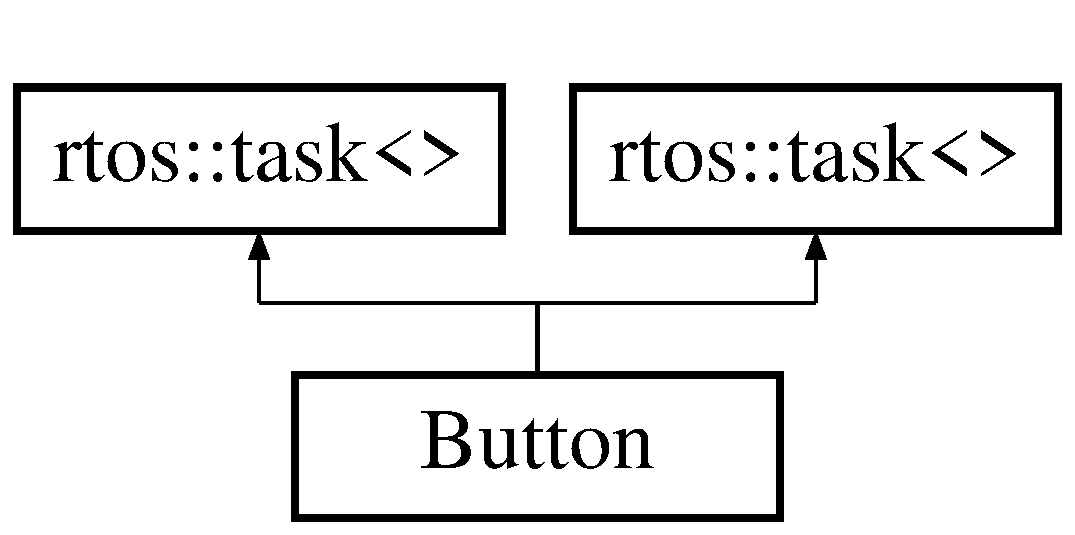
\includegraphics[height=2.000000cm]{class_button}
\end{center}
\end{figure}
\subsection*{Public Member Functions}
\begin{DoxyCompactItemize}
\item 
\mbox{\hyperlink{class_button_a7771486e8e6649ee30c85ab5580796da}{Button}} (const char $\ast$name, int priority, hwlib\+::pin\+\_\+in \&pin\+\_\+button, \mbox{\hyperlink{class_button_listener}{Button\+Listener}} \&listener, unsigned int buttonnumber)
\begin{DoxyCompactList}\small\item\em This is the constructor for a button. \end{DoxyCompactList}\item 
void \mbox{\hyperlink{class_button_a4cc671cc425acd0ee1b8f2f437cf40db}{main}} () override
\begin{DoxyCompactList}\small\item\em The main contains the state machine. \end{DoxyCompactList}\end{DoxyCompactItemize}


\subsection{Detailed Description}
This class is used to make a button object. 

\subsection{Constructor \& Destructor Documentation}
\mbox{\Hypertarget{class_button_a7771486e8e6649ee30c85ab5580796da}\label{class_button_a7771486e8e6649ee30c85ab5580796da}} 
\index{Button@{Button}!Button@{Button}}
\index{Button@{Button}!Button@{Button}}
\subsubsection{\texorpdfstring{Button()}{Button()}}
{\footnotesize\ttfamily Button\+::\+Button (\begin{DoxyParamCaption}\item[{const char $\ast$}]{name,  }\item[{int}]{priority,  }\item[{hwlib\+::pin\+\_\+in \&}]{pin\+\_\+button,  }\item[{\mbox{\hyperlink{class_button_listener}{Button\+Listener}} \&}]{listener,  }\item[{unsigned int}]{buttonnumber }\end{DoxyParamCaption})\hspace{0.3cm}{\ttfamily [inline]}}



This is the constructor for a button. 

The constructor expects a listener which is the class that owns the button. 

\subsection{Member Function Documentation}
\mbox{\Hypertarget{class_button_a4cc671cc425acd0ee1b8f2f437cf40db}\label{class_button_a4cc671cc425acd0ee1b8f2f437cf40db}} 
\index{Button@{Button}!main@{main}}
\index{main@{main}!Button@{Button}}
\subsubsection{\texorpdfstring{main()}{main()}}
{\footnotesize\ttfamily void Button\+::main (\begin{DoxyParamCaption}{ }\end{DoxyParamCaption})\hspace{0.3cm}{\ttfamily [inline]}, {\ttfamily [override]}}



The main contains the state machine. 

The main only consists of one state the wait\+\_\+for\+\_\+button\+\_\+press state. The state waits for a clock that gets called every 100 ms. When the clock is called the button pin gets checked for input. If there is a input the function buttonpressed in the listener gets called. 

The documentation for this class was generated from the following file\+:\begin{DoxyCompactItemize}
\item 
C\+:/ti-\/software/thema\+\_\+opdracht\+\_\+lasergame/\+Player/\mbox{\hyperlink{_button_8hpp}{Button.\+hpp}}\end{DoxyCompactItemize}

\hypertarget{class_button_listener}{}\section{Button\+Listener Class Reference}
\label{class_button_listener}\index{Button\+Listener@{Button\+Listener}}


A class containing the virtual button\+Pressed function.  




{\ttfamily \#include $<$Button\+Listener.\+hpp$>$}

Inheritance diagram for Button\+Listener\+:\begin{figure}[H]
\begin{center}
\leavevmode
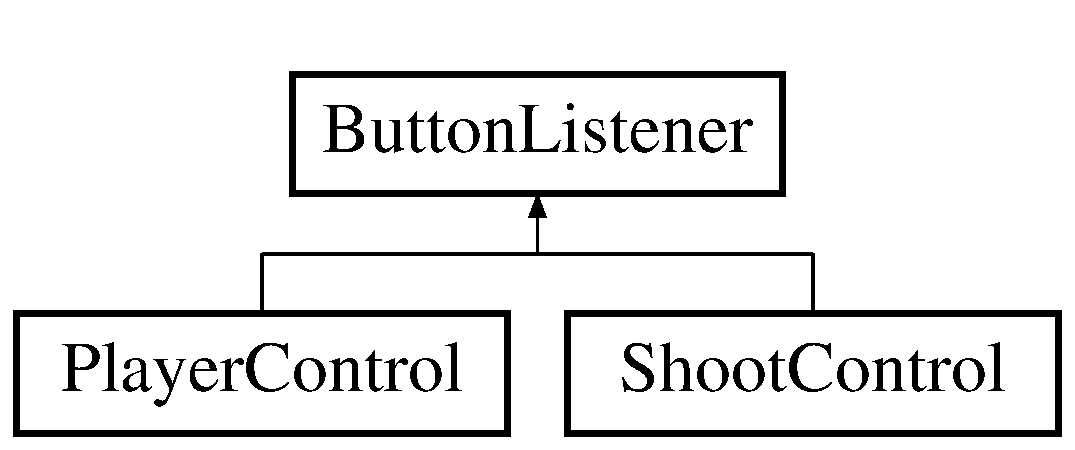
\includegraphics[height=2.000000cm]{class_button_listener}
\end{center}
\end{figure}
\subsection*{Public Member Functions}
\begin{DoxyCompactItemize}
\item 
\mbox{\Hypertarget{class_button_listener_a444f84514e359443020463edc129cd12}\label{class_button_listener_a444f84514e359443020463edc129cd12}} 
virtual void {\bfseries button\+Detected} ()=0
\item 
\mbox{\Hypertarget{class_button_listener_a669be11c0665a02e9501ee4ca03d8a8d}\label{class_button_listener_a669be11c0665a02e9501ee4ca03d8a8d}} 
virtual void \mbox{\hyperlink{class_button_listener_a669be11c0665a02e9501ee4ca03d8a8d}{button\+Pressed}} (unsigned int \&buttonnumber)=0
\begin{DoxyCompactList}\small\item\em This virtual function gets called by a button and gets overwritten in another class. \end{DoxyCompactList}\end{DoxyCompactItemize}


\subsection{Detailed Description}
A class containing the virtual button\+Pressed function. 

The documentation for this class was generated from the following files\+:\begin{DoxyCompactItemize}
\item 
C\+:/ti-\/software/thema\+\_\+opdracht\+\_\+lasergame/\+I\+R\+\_\+send/button\+\_\+listener.\+hpp\item 
C\+:/ti-\/software/thema\+\_\+opdracht\+\_\+lasergame/\+Player/\mbox{\hyperlink{_button_listener_8hpp}{Button\+Listener.\+hpp}}\end{DoxyCompactItemize}

\hypertarget{class_buzzer_control}{}\section{Buzzer\+Control Class Reference}
\label{class_buzzer_control}\index{Buzzer\+Control@{Buzzer\+Control}}


This class is used to control the buzzer.  




{\ttfamily \#include $<$Buzzer\+Control.\+hpp$>$}

Inheritance diagram for Buzzer\+Control\+:\begin{figure}[H]
\begin{center}
\leavevmode
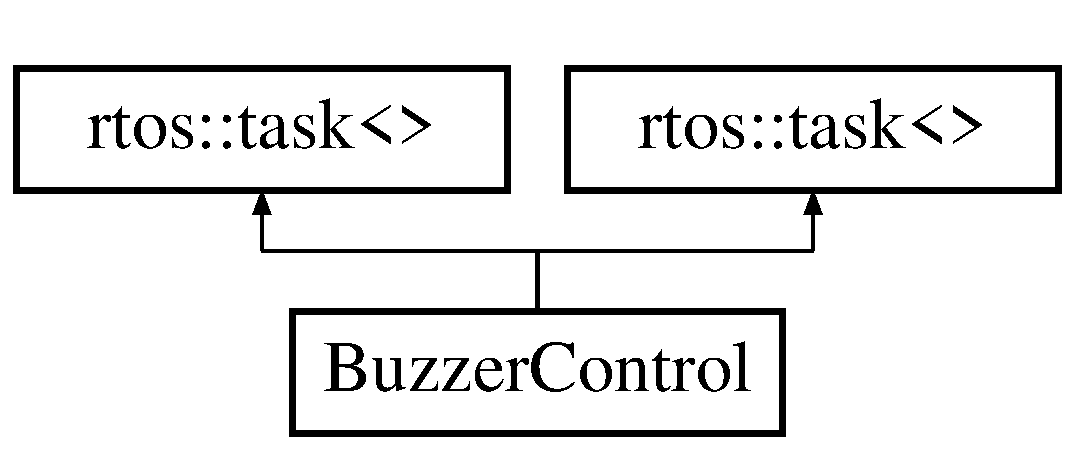
\includegraphics[height=2.000000cm]{class_buzzer_control}
\end{center}
\end{figure}
\subsection*{Public Member Functions}
\begin{DoxyCompactItemize}
\item 
\mbox{\hyperlink{class_buzzer_control_a25b3a51e33513aeeb0beb137463bbe70}{Buzzer\+Control}} (const char $\ast$name, int priority, hwlib\+::pin\+\_\+out \&buzz\+\_\+pin)
\begin{DoxyCompactList}\small\item\em This is the constructer for buzzer control. \end{DoxyCompactList}\item 
\mbox{\Hypertarget{class_buzzer_control_a2c485c8888d861efae8461a87a47685f}\label{class_buzzer_control_a2c485c8888d861efae8461a87a47685f}} 
void \mbox{\hyperlink{class_buzzer_control_a2c485c8888d861efae8461a87a47685f}{make\+Sound}} (int buzz\+\_\+length)
\begin{DoxyCompactList}\small\item\em This function writes the buzz\+\_\+length in the buzz\+\_\+pool and sets the buzz\+\_\+on\+\_\+flag. \end{DoxyCompactList}\item 
void \mbox{\hyperlink{class_buzzer_control_ae249e78ba5c0399e8b14091a0a8254eb}{main}} () override
\begin{DoxyCompactList}\small\item\em This is the state function for the buzzer. \end{DoxyCompactList}\end{DoxyCompactItemize}


\subsection{Detailed Description}
This class is used to control the buzzer. 

\subsection{Constructor \& Destructor Documentation}
\mbox{\Hypertarget{class_buzzer_control_a25b3a51e33513aeeb0beb137463bbe70}\label{class_buzzer_control_a25b3a51e33513aeeb0beb137463bbe70}} 
\index{Buzzer\+Control@{Buzzer\+Control}!Buzzer\+Control@{Buzzer\+Control}}
\index{Buzzer\+Control@{Buzzer\+Control}!Buzzer\+Control@{Buzzer\+Control}}
\subsubsection{\texorpdfstring{Buzzer\+Control()}{BuzzerControl()}}
{\footnotesize\ttfamily Buzzer\+Control\+::\+Buzzer\+Control (\begin{DoxyParamCaption}\item[{const char $\ast$}]{name,  }\item[{int}]{priority,  }\item[{hwlib\+::pin\+\_\+out \&}]{buzz\+\_\+pin }\end{DoxyParamCaption})\hspace{0.3cm}{\ttfamily [inline]}}



This is the constructer for buzzer control. 

The constructer wants a pin\+\_\+out buzz pin. 

\subsection{Member Function Documentation}
\mbox{\Hypertarget{class_buzzer_control_ae249e78ba5c0399e8b14091a0a8254eb}\label{class_buzzer_control_ae249e78ba5c0399e8b14091a0a8254eb}} 
\index{Buzzer\+Control@{Buzzer\+Control}!main@{main}}
\index{main@{main}!Buzzer\+Control@{Buzzer\+Control}}
\subsubsection{\texorpdfstring{main()}{main()}}
{\footnotesize\ttfamily void Buzzer\+Control\+::main (\begin{DoxyParamCaption}{ }\end{DoxyParamCaption})\hspace{0.3cm}{\ttfamily [inline]}, {\ttfamily [override]}}



This is the state function for the buzzer. 

This function has 3 states\+: I\+D\+LE, ON, O\+FF. If the state is I\+D\+LE, the function waits for the buzz\+\_\+on\+\_\+flag, then he reads the buzz\+\_\+pool, set the length timer and switch the state to ON. If the state is ON, buzz\+\_\+pin is set high, interval\+\_\+timer is set, he waits for the buzz\+\_\+interval\+\_\+timer and the state will be O\+FF. If the state is O\+FF, buzz\+\_\+pin is set low, interval\+\_\+timer is set and if event is the same as buzz\+\_\+length\+\_\+timer, the state will be I\+D\+LE. If event is the ame as buzz\+\_\+interval\+\_\+timer, the state will be ON. 

The documentation for this class was generated from the following file\+:\begin{DoxyCompactItemize}
\item 
C\+:/ti-\/software/thema\+\_\+opdracht\+\_\+lasergame/\+Player/\mbox{\hyperlink{_buzzer_control_8hpp}{Buzzer\+Control.\+hpp}}\end{DoxyCompactItemize}

\hypertarget{class_display_control}{}\section{Display\+Control Class Reference}
\label{class_display_control}\index{Display\+Control@{Display\+Control}}


This class is used to show the command value on the screen.  




{\ttfamily \#include $<$Display\+Control.\+hpp$>$}

Inheritance diagram for Display\+Control\+:\begin{figure}[H]
\begin{center}
\leavevmode
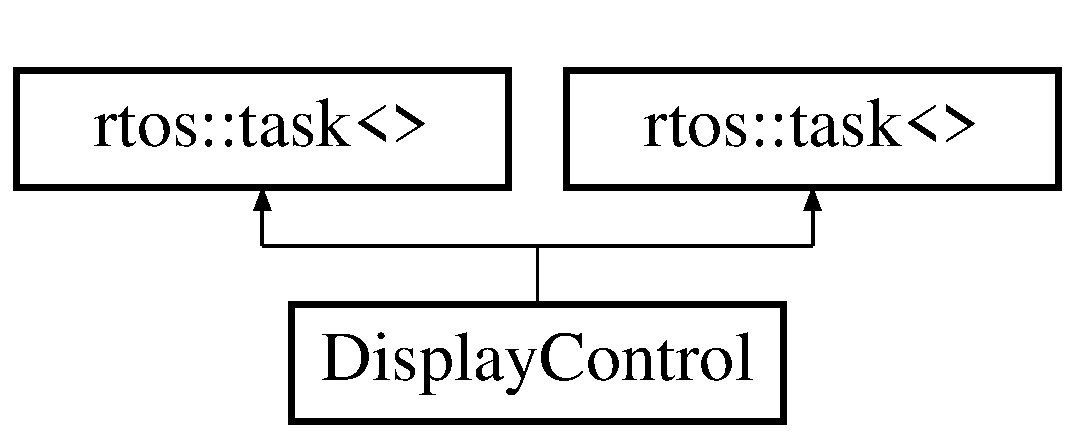
\includegraphics[height=2.000000cm]{class_display_control}
\end{center}
\end{figure}
\subsection*{Public Member Functions}
\begin{DoxyCompactItemize}
\item 
\mbox{\hyperlink{class_display_control_a5a24ccc28d6984bda6871ef6d0e4af3f}{Display\+Control}} (const char $\ast$name, int priority, hwlib\+::glcd\+\_\+oled \&display)
\begin{DoxyCompactList}\small\item\em This is the constructor for a display. \end{DoxyCompactList}\item 
\mbox{\Hypertarget{class_display_control_a78b3ace358fc199a76e00148115f449d}\label{class_display_control_a78b3ace358fc199a76e00148115f449d}} 
void \mbox{\hyperlink{class_display_control_a78b3ace358fc199a76e00148115f449d}{show\+Command}} (uint8\+\_\+t value)
\begin{DoxyCompactList}\small\item\em This function sets a flag en writes the value in the command\+\_\+pool. \end{DoxyCompactList}\item 
\mbox{\Hypertarget{class_display_control_aa231d63d18b09506e0c766999f480579}\label{class_display_control_aa231d63d18b09506e0c766999f480579}} 
void \mbox{\hyperlink{class_display_control_aa231d63d18b09506e0c766999f480579}{clear}} ()
\begin{DoxyCompactList}\small\item\em This function sets a flag to clear the screen. \end{DoxyCompactList}\item 
void \mbox{\hyperlink{class_display_control_ae2d8d0f502941d859639fd46ddd8924b}{update\+Command\+Value}} (uint8\+\_\+t value)
\begin{DoxyCompactList}\small\item\em This function updates the command value on the screen. \end{DoxyCompactList}\item 
\mbox{\Hypertarget{class_display_control_a01207b2034dc3946856496bf2e4d39b6}\label{class_display_control_a01207b2034dc3946856496bf2e4d39b6}} 
void \mbox{\hyperlink{class_display_control_a01207b2034dc3946856496bf2e4d39b6}{clear\+Command\+Value}} ()
\begin{DoxyCompactList}\small\item\em This function clears the command value on the screen. \end{DoxyCompactList}\item 
void \mbox{\hyperlink{class_display_control_a9707c32249e0a648afc2def818900f30}{main}} () override
\begin{DoxyCompactList}\small\item\em This is the state function for the display class. \end{DoxyCompactList}\item 
\mbox{\hyperlink{class_display_control_a5a24ccc28d6984bda6871ef6d0e4af3f}{Display\+Control}} (const char $\ast$name, int priority, hwlib\+::glcd\+\_\+oled \&display)
\begin{DoxyCompactList}\small\item\em This is the constructor for a display. \end{DoxyCompactList}\item 
\mbox{\Hypertarget{class_display_control_a78b3ace358fc199a76e00148115f449d}\label{class_display_control_a78b3ace358fc199a76e00148115f449d}} 
void \mbox{\hyperlink{class_display_control_a78b3ace358fc199a76e00148115f449d}{show\+Command}} (uint8\+\_\+t value)
\begin{DoxyCompactList}\small\item\em This function sets a flag en writes the value in the command\+\_\+pool. \end{DoxyCompactList}\item 
\mbox{\Hypertarget{class_display_control_adcdd7237b9510e9cb9b2aff9d695ad2e}\label{class_display_control_adcdd7237b9510e9cb9b2aff9d695ad2e}} 
void \mbox{\hyperlink{class_display_control_adcdd7237b9510e9cb9b2aff9d695ad2e}{show\+Countdown}} (uint8\+\_\+t value)
\begin{DoxyCompactList}\small\item\em This function sets a flag en writes the value in the countdown\+\_\+pool. \end{DoxyCompactList}\item 
\mbox{\Hypertarget{class_display_control_aee4d1de8dc9b2aab72685cef2ce42d92}\label{class_display_control_aee4d1de8dc9b2aab72685cef2ce42d92}} 
void \mbox{\hyperlink{class_display_control_aee4d1de8dc9b2aab72685cef2ce42d92}{show\+Deaths}} (uint8\+\_\+t value)
\begin{DoxyCompactList}\small\item\em This function sets a flag en writes the value in the deaths\+\_\+pool. \end{DoxyCompactList}\item 
\mbox{\Hypertarget{class_display_control_a6b4ed1ee72406c1ab082b7c6cf900001}\label{class_display_control_a6b4ed1ee72406c1ab082b7c6cf900001}} 
void \mbox{\hyperlink{class_display_control_a6b4ed1ee72406c1ab082b7c6cf900001}{show\+Ammo}} (uint8\+\_\+t value)
\begin{DoxyCompactList}\small\item\em This function sets a flag en writes the value in the ammo\+\_\+pool. \end{DoxyCompactList}\item 
\mbox{\Hypertarget{class_display_control_a4cb0b2e7b72f7267531ffb0470216651}\label{class_display_control_a4cb0b2e7b72f7267531ffb0470216651}} 
void \mbox{\hyperlink{class_display_control_a4cb0b2e7b72f7267531ffb0470216651}{show\+Health}} (uint8\+\_\+t value)
\begin{DoxyCompactList}\small\item\em This function sets a flag en writes the value in the health\+\_\+pool. \end{DoxyCompactList}\item 
\mbox{\Hypertarget{class_display_control_a1f33d5376aee69c307444fef969a1870}\label{class_display_control_a1f33d5376aee69c307444fef969a1870}} 
void \mbox{\hyperlink{class_display_control_a1f33d5376aee69c307444fef969a1870}{show\+Player}} (uint8\+\_\+t value)
\begin{DoxyCompactList}\small\item\em This function sets a flag en writes the value in the player\+\_\+pool. \end{DoxyCompactList}\item 
\mbox{\Hypertarget{class_display_control_a4be28ed55f806917cf4cb7bab68ea6eb}\label{class_display_control_a4be28ed55f806917cf4cb7bab68ea6eb}} 
void \mbox{\hyperlink{class_display_control_a4be28ed55f806917cf4cb7bab68ea6eb}{show\+Weapon}} (const char $\ast$value)
\begin{DoxyCompactList}\small\item\em This function sets a flag en writes the value in the weapon\+\_\+pool. \end{DoxyCompactList}\item 
\mbox{\Hypertarget{class_display_control_ae2d8d0f502941d859639fd46ddd8924b}\label{class_display_control_ae2d8d0f502941d859639fd46ddd8924b}} 
void \mbox{\hyperlink{class_display_control_ae2d8d0f502941d859639fd46ddd8924b}{update\+Command\+Value}} (uint8\+\_\+t value)
\begin{DoxyCompactList}\small\item\em This function updates the command value on the screen. \end{DoxyCompactList}\item 
\mbox{\Hypertarget{class_display_control_a7a566545dbdd6834307d27de99a221d6}\label{class_display_control_a7a566545dbdd6834307d27de99a221d6}} 
void \mbox{\hyperlink{class_display_control_a7a566545dbdd6834307d27de99a221d6}{update\+Countdown\+Value}} (uint8\+\_\+t value)
\begin{DoxyCompactList}\small\item\em This function updates the countdown value on the screen. \end{DoxyCompactList}\item 
\mbox{\Hypertarget{class_display_control_a6bb416767f43144827fa5bf6ecece4a9}\label{class_display_control_a6bb416767f43144827fa5bf6ecece4a9}} 
void \mbox{\hyperlink{class_display_control_a6bb416767f43144827fa5bf6ecece4a9}{update\+Deaths\+Value}} (uint8\+\_\+t value)
\begin{DoxyCompactList}\small\item\em This function updates the deaths value on the screen. \end{DoxyCompactList}\item 
\mbox{\Hypertarget{class_display_control_aa54c7b984287e6a694ea83a3cb3d8ece}\label{class_display_control_aa54c7b984287e6a694ea83a3cb3d8ece}} 
void \mbox{\hyperlink{class_display_control_aa54c7b984287e6a694ea83a3cb3d8ece}{update\+Ammo\+Value}} (uint8\+\_\+t value)
\begin{DoxyCompactList}\small\item\em This function updates the ammo value on the screen. \end{DoxyCompactList}\item 
\mbox{\Hypertarget{class_display_control_a1d61b517063ca3f3dd36d2b7eb3ef909}\label{class_display_control_a1d61b517063ca3f3dd36d2b7eb3ef909}} 
void \mbox{\hyperlink{class_display_control_a1d61b517063ca3f3dd36d2b7eb3ef909}{update\+Healt\+Value}} (uint8\+\_\+t value)
\begin{DoxyCompactList}\small\item\em This function updates the health value on the screen. \end{DoxyCompactList}\item 
\mbox{\Hypertarget{class_display_control_ad6107e04362c907da6a64b73bcc9e795}\label{class_display_control_ad6107e04362c907da6a64b73bcc9e795}} 
void \mbox{\hyperlink{class_display_control_ad6107e04362c907da6a64b73bcc9e795}{update\+Player\+Value}} (uint8\+\_\+t value)
\begin{DoxyCompactList}\small\item\em This function updates the player value on the screen. \end{DoxyCompactList}\item 
\mbox{\Hypertarget{class_display_control_ae343066ad92148ddc6cd9f253993d4b4}\label{class_display_control_ae343066ad92148ddc6cd9f253993d4b4}} 
void \mbox{\hyperlink{class_display_control_ae343066ad92148ddc6cd9f253993d4b4}{update\+Weapon\+Value}} (const char $\ast$value)
\begin{DoxyCompactList}\small\item\em This function updates the weapon value on the screen. \end{DoxyCompactList}\item 
void \mbox{\hyperlink{class_display_control_a9707c32249e0a648afc2def818900f30}{main}} () override
\begin{DoxyCompactList}\small\item\em This is the state function for the display class. \end{DoxyCompactList}\end{DoxyCompactItemize}


\subsection{Detailed Description}
This class is used to show the command value on the screen. 

\subsection{Constructor \& Destructor Documentation}
\mbox{\Hypertarget{class_display_control_a5a24ccc28d6984bda6871ef6d0e4af3f}\label{class_display_control_a5a24ccc28d6984bda6871ef6d0e4af3f}} 
\index{Display\+Control@{Display\+Control}!Display\+Control@{Display\+Control}}
\index{Display\+Control@{Display\+Control}!Display\+Control@{Display\+Control}}
\subsubsection{\texorpdfstring{Display\+Control()}{DisplayControl()}\hspace{0.1cm}{\footnotesize\ttfamily [1/2]}}
{\footnotesize\ttfamily Display\+Control\+::\+Display\+Control (\begin{DoxyParamCaption}\item[{const char $\ast$}]{name,  }\item[{int}]{priority,  }\item[{hwlib\+::glcd\+\_\+oled \&}]{display }\end{DoxyParamCaption})\hspace{0.3cm}{\ttfamily [inline]}}



This is the constructor for a display. 

The constructor expects a display. \mbox{\Hypertarget{class_display_control_a5a24ccc28d6984bda6871ef6d0e4af3f}\label{class_display_control_a5a24ccc28d6984bda6871ef6d0e4af3f}} 
\index{Display\+Control@{Display\+Control}!Display\+Control@{Display\+Control}}
\index{Display\+Control@{Display\+Control}!Display\+Control@{Display\+Control}}
\subsubsection{\texorpdfstring{Display\+Control()}{DisplayControl()}\hspace{0.1cm}{\footnotesize\ttfamily [2/2]}}
{\footnotesize\ttfamily Display\+Control\+::\+Display\+Control (\begin{DoxyParamCaption}\item[{const char $\ast$}]{name,  }\item[{int}]{priority,  }\item[{hwlib\+::glcd\+\_\+oled \&}]{display }\end{DoxyParamCaption})\hspace{0.3cm}{\ttfamily [inline]}}



This is the constructor for a display. 

The constructor expects a display. 

\subsection{Member Function Documentation}
\mbox{\Hypertarget{class_display_control_a9707c32249e0a648afc2def818900f30}\label{class_display_control_a9707c32249e0a648afc2def818900f30}} 
\index{Display\+Control@{Display\+Control}!main@{main}}
\index{main@{main}!Display\+Control@{Display\+Control}}
\subsubsection{\texorpdfstring{main()}{main()}\hspace{0.1cm}{\footnotesize\ttfamily [1/2]}}
{\footnotesize\ttfamily void Display\+Control\+::main (\begin{DoxyParamCaption}{ }\end{DoxyParamCaption})\hspace{0.3cm}{\ttfamily [inline]}, {\ttfamily [override]}}



This is the state function for the display class. 

This function has one state\+: W\+A\+I\+T\+\_\+\+F\+O\+R\+\_\+\+M\+E\+S\+S\+A\+GE. The function will wait for the display\+\_\+command\+\_\+flag and will wait and call a function where he will read the pool. Else if he will wait for the clear\+\_\+flag and will call a function. \mbox{\Hypertarget{class_display_control_a9707c32249e0a648afc2def818900f30}\label{class_display_control_a9707c32249e0a648afc2def818900f30}} 
\index{Display\+Control@{Display\+Control}!main@{main}}
\index{main@{main}!Display\+Control@{Display\+Control}}
\subsubsection{\texorpdfstring{main()}{main()}\hspace{0.1cm}{\footnotesize\ttfamily [2/2]}}
{\footnotesize\ttfamily void Display\+Control\+::main (\begin{DoxyParamCaption}{ }\end{DoxyParamCaption})\hspace{0.3cm}{\ttfamily [inline]}, {\ttfamily [override]}}



This is the state function for the display class. 

This function has one state\+: W\+A\+I\+T\+\_\+\+F\+O\+R\+\_\+\+M\+E\+S\+S\+A\+GE. If event is the same as display\+\_\+command\+\_\+flag, the function update\+Command\+Value with as parameter the readen comman\+\_\+pool value. If event is the same as display\+\_\+countdown\+\_\+flag, the function update\+Countdown\+Value with as parameter the readen countdown\+\_\+pool value. If event is the same as display\+\_\+deaths\+\_\+flag, the function update\+Deaths\+Value with as parameter the readen deaths\+\_\+pool value. If event is the same as display\+\_\+ammo\+\_\+flag, the function update\+Ammo\+Value with as parameter the readen ammo\+\_\+pool value. If event is the same as display\+\_\+health\+\_\+flag, the function update\+Health\+Value with as parameter the readen health\+\_\+pool value. If event is the same as display\+\_\+player\+\_\+flag, the function update\+Player\+Value with as parameter the readen player\+\_\+pool value. If event is the same as display\+\_\+weapon\+\_\+flag, the function update\+Weapon\+Value with as parameter the readen Weapon\+\_\+pool value. \mbox{\Hypertarget{class_display_control_ae2d8d0f502941d859639fd46ddd8924b}\label{class_display_control_ae2d8d0f502941d859639fd46ddd8924b}} 
\index{Display\+Control@{Display\+Control}!update\+Command\+Value@{update\+Command\+Value}}
\index{update\+Command\+Value@{update\+Command\+Value}!Display\+Control@{Display\+Control}}
\subsubsection{\texorpdfstring{update\+Command\+Value()}{updateCommandValue()}}
{\footnotesize\ttfamily void Display\+Control\+::update\+Command\+Value (\begin{DoxyParamCaption}\item[{uint8\+\_\+t}]{value }\end{DoxyParamCaption})\hspace{0.3cm}{\ttfamily [inline]}}



This function updates the command value on the screen. 

If the value is 42, the function makes a star of it. This is special for the star on the gamepad. Else the function will print the int value on the screen. 

The documentation for this class was generated from the following file\+:\begin{DoxyCompactItemize}
\item 
C\+:/ti-\/software/thema\+\_\+opdracht\+\_\+lasergame/\+Gameleader/\mbox{\hyperlink{_gameleader_2_display_control_8hpp}{Display\+Control.\+hpp}}\end{DoxyCompactItemize}

\hypertarget{class_game_leader}{}\section{Game\+Leader Class Reference}
\label{class_game_leader}\index{Game\+Leader@{Game\+Leader}}


This class is used to make the game.  




{\ttfamily \#include $<$Game\+Leader.\+hpp$>$}

Inheritance diagram for Game\+Leader\+:\begin{figure}[H]
\begin{center}
\leavevmode
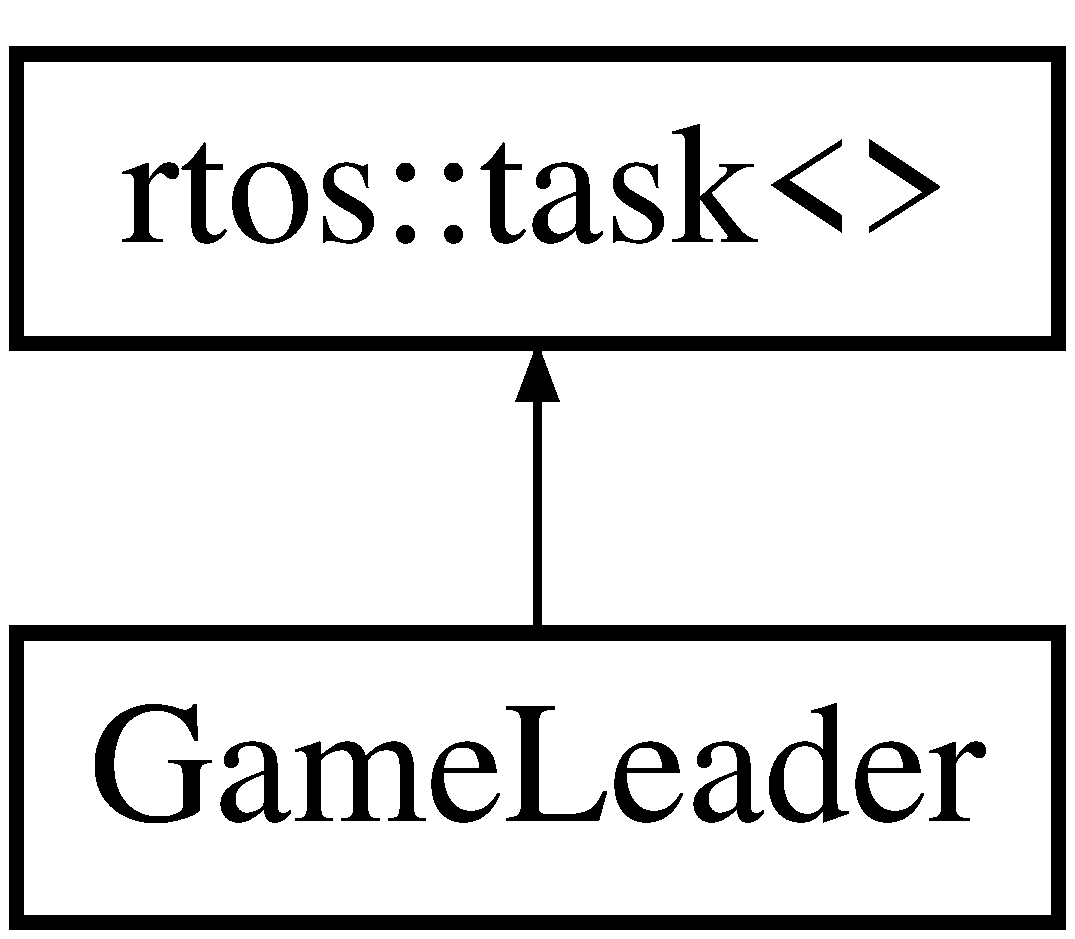
\includegraphics[height=2.000000cm]{class_game_leader}
\end{center}
\end{figure}
\subsection*{Public Member Functions}
\begin{DoxyCompactItemize}
\item 
\mbox{\hyperlink{class_game_leader_a37f89b9731c43cb875207ebbbcdcc96f}{Game\+Leader}} (const char $\ast$name, int priority, \mbox{\hyperlink{class_send_control}{Send\+Control}} \&send\+\_\+control)
\begin{DoxyCompactList}\small\item\em This is the constructor for the \mbox{\hyperlink{class_game_leader}{Game\+Leader}}. \end{DoxyCompactList}\item 
\mbox{\Hypertarget{class_game_leader_a704a13665a65f4528ed3022111c468e2}\label{class_game_leader_a704a13665a65f4528ed3022111c468e2}} 
void \mbox{\hyperlink{class_game_leader_a704a13665a65f4528ed3022111c468e2}{set\+Game\+Length}} (uint8\+\_\+t length)
\begin{DoxyCompactList}\small\item\em This function writes the given length in the game\+\_\+length\+\_\+pool and sets the game\+\_\+length\+\_\+flag. \end{DoxyCompactList}\item 
\mbox{\Hypertarget{class_game_leader_a42849b606a56928126bc915b56695b38}\label{class_game_leader_a42849b606a56928126bc915b56695b38}} 
void \mbox{\hyperlink{class_game_leader_a42849b606a56928126bc915b56695b38}{start\+Game}} ()
\begin{DoxyCompactList}\small\item\em This function sets the start\+\_\+game\+\_\+flag. \end{DoxyCompactList}\item 
void \mbox{\hyperlink{class_game_leader_a83c1a53edf86e4a740c6e4a08f022f36}{main}} () override
\begin{DoxyCompactList}\small\item\em This is the state function for the \mbox{\hyperlink{class_game_leader}{Game\+Leader}} class. \end{DoxyCompactList}\end{DoxyCompactItemize}


\subsection{Detailed Description}
This class is used to make the game. 

\subsection{Constructor \& Destructor Documentation}
\mbox{\Hypertarget{class_game_leader_a37f89b9731c43cb875207ebbbcdcc96f}\label{class_game_leader_a37f89b9731c43cb875207ebbbcdcc96f}} 
\index{Game\+Leader@{Game\+Leader}!Game\+Leader@{Game\+Leader}}
\index{Game\+Leader@{Game\+Leader}!Game\+Leader@{Game\+Leader}}
\subsubsection{\texorpdfstring{Game\+Leader()}{GameLeader()}}
{\footnotesize\ttfamily Game\+Leader\+::\+Game\+Leader (\begin{DoxyParamCaption}\item[{const char $\ast$}]{name,  }\item[{int}]{priority,  }\item[{\mbox{\hyperlink{class_send_control}{Send\+Control}} \&}]{send\+\_\+control }\end{DoxyParamCaption})\hspace{0.3cm}{\ttfamily [inline]}}



This is the constructor for the \mbox{\hyperlink{class_game_leader}{Game\+Leader}}. 

The constructor expects a \mbox{\hyperlink{class_send_control}{Send\+Control}} as parameter. 

\subsection{Member Function Documentation}
\mbox{\Hypertarget{class_game_leader_a83c1a53edf86e4a740c6e4a08f022f36}\label{class_game_leader_a83c1a53edf86e4a740c6e4a08f022f36}} 
\index{Game\+Leader@{Game\+Leader}!main@{main}}
\index{main@{main}!Game\+Leader@{Game\+Leader}}
\subsubsection{\texorpdfstring{main()}{main()}}
{\footnotesize\ttfamily void Game\+Leader\+::main (\begin{DoxyParamCaption}{ }\end{DoxyParamCaption})\hspace{0.3cm}{\ttfamily [inline]}, {\ttfamily [override]}}



This is the state function for the \mbox{\hyperlink{class_game_leader}{Game\+Leader}} class. 

This function has one state\+: W\+A\+I\+T\+I\+N\+G\+\_\+\+F\+O\+R\+\_\+\+C\+O\+M\+M\+A\+ND. The function waits for game\+\_\+length\+\_\+flag and then he will send the value in the game\+\_\+length\+\_\+pool. Else he will wait for the start\+\_\+game\+\_\+flag en then he will send the start\+\_\+game\+\_\+value. 

The documentation for this class was generated from the following file\+:\begin{DoxyCompactItemize}
\item 
C\+:/ti-\/software/thema\+\_\+opdracht\+\_\+lasergame/\+Gameleader/\mbox{\hyperlink{_game_leader_8hpp}{Game\+Leader.\+hpp}}\end{DoxyCompactItemize}

\hypertarget{class_game_logs}{}\section{Game\+Logs Class Reference}
\label{class_game_logs}\index{Game\+Logs@{Game\+Logs}}
\subsection*{Public Member Functions}
\begin{DoxyCompactItemize}
\item 
\mbox{\Hypertarget{class_game_logs_aff50867c6abefacf3d80180015f94e70}\label{class_game_logs_aff50867c6abefacf3d80180015f94e70}} 
void {\bfseries add\+Log} (uint8\+\_\+t player, const char $\ast$weapon)
\item 
\mbox{\Hypertarget{class_game_logs_a2af40236b4dc804f4dc0fac938d0bfd9}\label{class_game_logs_a2af40236b4dc804f4dc0fac938d0bfd9}} 
void {\bfseries print\+Log} ()
\item 
\mbox{\Hypertarget{class_game_logs_ab645b6718f2d5ee716c8b4df4dddf561}\label{class_game_logs_ab645b6718f2d5ee716c8b4df4dddf561}} 
void {\bfseries clear\+Logs} ()
\end{DoxyCompactItemize}


The documentation for this class was generated from the following file\+:\begin{DoxyCompactItemize}
\item 
C\+:/ti-\/software/thema\+\_\+opdracht\+\_\+lasergame/\+Gameleader/Game\+Logs.\+hpp\end{DoxyCompactItemize}

\hypertarget{structir__msg}{}\section{ir\+\_\+msg Struct Reference}
\label{structir__msg}\index{ir\+\_\+msg@{ir\+\_\+msg}}


This struct gets used to split the message in two parts.  




{\ttfamily \#include $<$Msg\+Listener.\+hpp$>$}

\subsection*{Public Attributes}
\begin{DoxyCompactItemize}
\item 
\mbox{\Hypertarget{structir__msg_a1aba19ec600f05dbf3e20cd94585f2b7}\label{structir__msg_a1aba19ec600f05dbf3e20cd94585f2b7}} 
uint8\+\_\+t {\bfseries player}
\item 
\mbox{\Hypertarget{structir__msg_a186ea1a98c46be88a9664b2ca285566f}\label{structir__msg_a186ea1a98c46be88a9664b2ca285566f}} 
uint8\+\_\+t {\bfseries data}
\end{DoxyCompactItemize}


\subsection{Detailed Description}
This struct gets used to split the message in two parts. 

The message gets split into the player part and the data part. 

The documentation for this struct was generated from the following file\+:\begin{DoxyCompactItemize}
\item 
C\+:/ti-\/software/thema\+\_\+opdracht\+\_\+lasergame/\+Player/\mbox{\hyperlink{_msg_listener_8hpp}{Msg\+Listener.\+hpp}}\end{DoxyCompactItemize}

\hypertarget{class_i_r_control}{}\section{I\+R\+Control Class Reference}
\label{class_i_r_control}\index{I\+R\+Control@{I\+R\+Control}}
Inheritance diagram for I\+R\+Control\+:\begin{figure}[H]
\begin{center}
\leavevmode
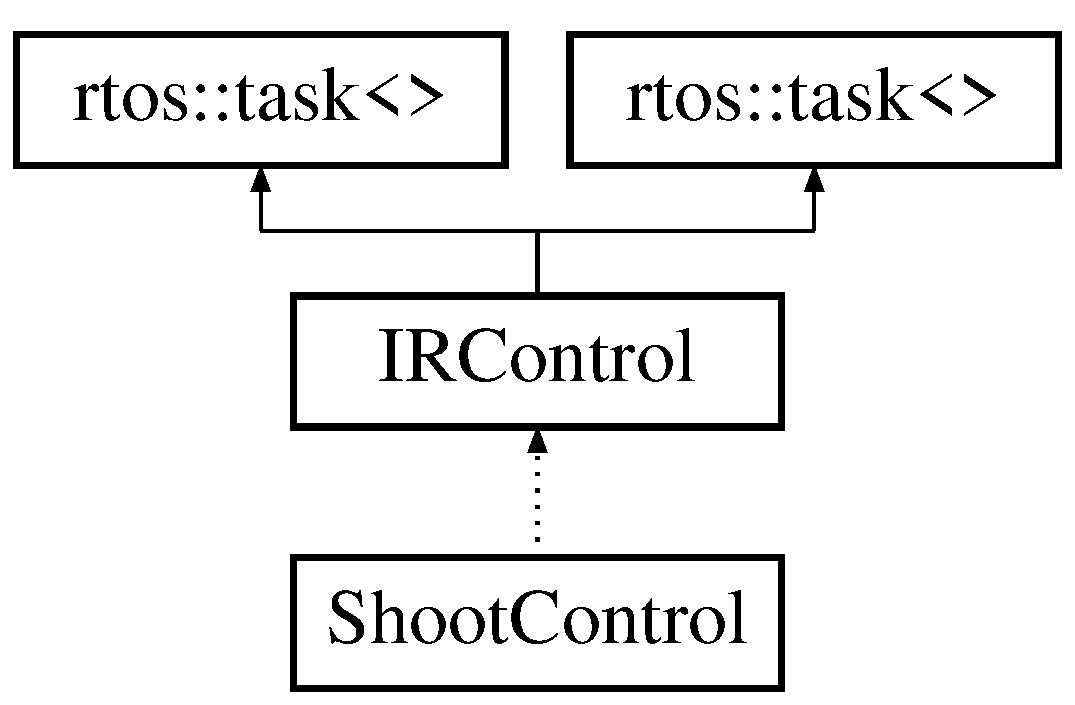
\includegraphics[height=2.000000cm]{class_i_r_control}
\end{center}
\end{figure}
\subsection*{Public Member Functions}
\begin{DoxyCompactItemize}
\item 
\mbox{\Hypertarget{class_i_r_control_ac16a197b453b4bd18874dbc1ef2d3cf4}\label{class_i_r_control_ac16a197b453b4bd18874dbc1ef2d3cf4}} 
void {\bfseries send} (const uint16\+\_\+t \&data)
\item 
\mbox{\Hypertarget{class_i_r_control_a12e0082a899fc811fa70c5cbe59e18d0}\label{class_i_r_control_a12e0082a899fc811fa70c5cbe59e18d0}} 
void {\bfseries pulse} (bool data)
\end{DoxyCompactItemize}


The documentation for this class was generated from the following file\+:\begin{DoxyCompactItemize}
\item 
C\+:/ti-\/software/thema\+\_\+opdracht\+\_\+lasergame/\+I\+R\+\_\+send/I\+R\+Control.\+hpp\end{DoxyCompactItemize}

\hypertarget{class_keypad}{}\section{Keypad Class Reference}
\label{class_keypad}\index{Keypad@{Keypad}}


In this class you can find the pin setup and initialize the characters.  




{\ttfamily \#include $<$Keypad.\+hpp$>$}

Inheritance diagram for Keypad\+:\begin{figure}[H]
\begin{center}
\leavevmode
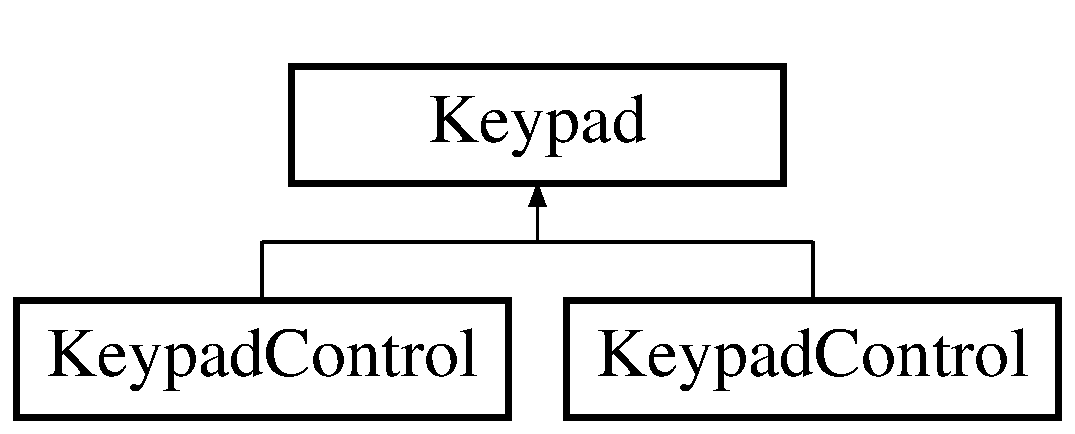
\includegraphics[height=2.000000cm]{class_keypad}
\end{center}
\end{figure}
\subsection*{Public Member Functions}
\begin{DoxyCompactItemize}
\item 
\mbox{\Hypertarget{class_keypad_ade2df731c6751f21bbf745b276cb7208}\label{class_keypad_ade2df731c6751f21bbf745b276cb7208}} 
char \mbox{\hyperlink{class_keypad_ade2df731c6751f21bbf745b276cb7208}{getc}} ()
\begin{DoxyCompactList}\small\item\em This function returns the pressed character. \end{DoxyCompactList}\end{DoxyCompactItemize}


\subsection{Detailed Description}
In this class you can find the pin setup and initialize the characters. 

The documentation for this class was generated from the following file\+:\begin{DoxyCompactItemize}
\item 
C\+:/ti-\/software/thema\+\_\+opdracht\+\_\+lasergame/\+Player/\mbox{\hyperlink{_keypad_8hpp}{Keypad.\+hpp}}\end{DoxyCompactItemize}

\hypertarget{class_keypad_control}{}\section{Keypad\+Control Class Reference}
\label{class_keypad_control}\index{Keypad\+Control@{Keypad\+Control}}


This class is used to control the keypad.  




{\ttfamily \#include $<$Keypad\+Control.\+hpp$>$}

Inheritance diagram for Keypad\+Control\+:\begin{figure}[H]
\begin{center}
\leavevmode
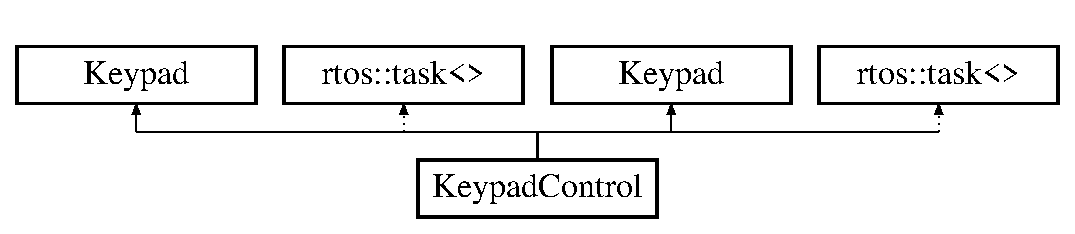
\includegraphics[height=2.000000cm]{class_keypad_control}
\end{center}
\end{figure}
\subsection*{Public Member Functions}
\begin{DoxyCompactItemize}
\item 
\mbox{\hyperlink{class_keypad_control_a4de1bb3018f819011222461d64aa2d67}{Keypad\+Control}} (const char $\ast$name, int priority, \mbox{\hyperlink{class_display_control}{Display\+Control}} \&display\+\_\+control, \mbox{\hyperlink{class_player_control}{Player\+Control}} \&player\+\_\+control, \mbox{\hyperlink{class_weapon}{Weapon}} \&weapon, \mbox{\hyperlink{class_player_data}{Player\+Data}} \&player\+\_\+data)
\begin{DoxyCompactList}\small\item\em This is the constructor for keypad control. \end{DoxyCompactList}\item 
void \mbox{\hyperlink{class_keypad_control_a66ec8a33eceb20d5d1d243c270c3718b}{main}} () override
\begin{DoxyCompactList}\small\item\em This is the state function for the keypad class. \end{DoxyCompactList}\end{DoxyCompactItemize}


\subsection{Detailed Description}
This class is used to control the keypad. 

\subsection{Constructor \& Destructor Documentation}
\mbox{\Hypertarget{class_keypad_control_a4de1bb3018f819011222461d64aa2d67}\label{class_keypad_control_a4de1bb3018f819011222461d64aa2d67}} 
\index{Keypad\+Control@{Keypad\+Control}!Keypad\+Control@{Keypad\+Control}}
\index{Keypad\+Control@{Keypad\+Control}!Keypad\+Control@{Keypad\+Control}}
\subsubsection{\texorpdfstring{Keypad\+Control()}{KeypadControl()}}
{\footnotesize\ttfamily Keypad\+Control\+::\+Keypad\+Control (\begin{DoxyParamCaption}\item[{const char $\ast$}]{name,  }\item[{int}]{priority,  }\item[{\mbox{\hyperlink{class_display_control}{Display\+Control}} \&}]{display\+\_\+control,  }\item[{\mbox{\hyperlink{class_player_control}{Player\+Control}} \&}]{player\+\_\+control,  }\item[{\mbox{\hyperlink{class_weapon}{Weapon}} \&}]{weapon,  }\item[{\mbox{\hyperlink{class_player_data}{Player\+Data}} \&}]{player\+\_\+data }\end{DoxyParamCaption})\hspace{0.3cm}{\ttfamily [inline]}}



This is the constructor for keypad control. 

The constructor needs \mbox{\hyperlink{class_display_control}{Display\+Control}}, \mbox{\hyperlink{class_player_control}{Player\+Control}}, \mbox{\hyperlink{class_weapon}{Weapon}}, \mbox{\hyperlink{class_player_data}{Player\+Data}}. 

\subsection{Member Function Documentation}
\mbox{\Hypertarget{class_keypad_control_a66ec8a33eceb20d5d1d243c270c3718b}\label{class_keypad_control_a66ec8a33eceb20d5d1d243c270c3718b}} 
\index{Keypad\+Control@{Keypad\+Control}!main@{main}}
\index{main@{main}!Keypad\+Control@{Keypad\+Control}}
\subsubsection{\texorpdfstring{main()}{main()}}
{\footnotesize\ttfamily void Keypad\+Control\+::main (\begin{DoxyParamCaption}{ }\end{DoxyParamCaption})\hspace{0.3cm}{\ttfamily [inline]}, {\ttfamily [override]}}



This is the state function for the keypad class. 

This function has 3 states\+: I\+D\+LE, P\+L\+A\+Y\+ER and W\+E\+A\+P\+ON. If the state is I\+D\+LE, the function waits for the receive\+\_\+clock and will look for the pressed key.\+If the pressed key is A then the state will be P\+L\+A\+Y\+ER. Else if the pressed key is B, the state will be W\+E\+A\+P\+ON. If the state is P\+L\+A\+Y\+ER, the function waits for the receive\+\_\+clock and will look for the pressed key. If keyvalue is a number but not 0, the set\+Player\+Number and Show\+Command functions will be called and the state will be I\+D\+LE. If state is W\+E\+A\+P\+ON, the function will wait for the receive\+\_\+clock and will look for the pressed key. If keyvalue is a number but not 0, the set\+Weapon and show\+Command functions will be called and the state will be I\+D\+LE. 

The documentation for this class was generated from the following file\+:\begin{DoxyCompactItemize}
\item 
C\+:/ti-\/software/thema\+\_\+opdracht\+\_\+lasergame/\+Player/\mbox{\hyperlink{_keypad_control_8hpp}{Keypad\+Control.\+hpp}}\end{DoxyCompactItemize}

\hypertarget{classmsg__decoder}{}\section{msg\+\_\+decoder Class Reference}
\label{classmsg__decoder}\index{msg\+\_\+decoder@{msg\+\_\+decoder}}
Inheritance diagram for msg\+\_\+decoder\+:\begin{figure}[H]
\begin{center}
\leavevmode
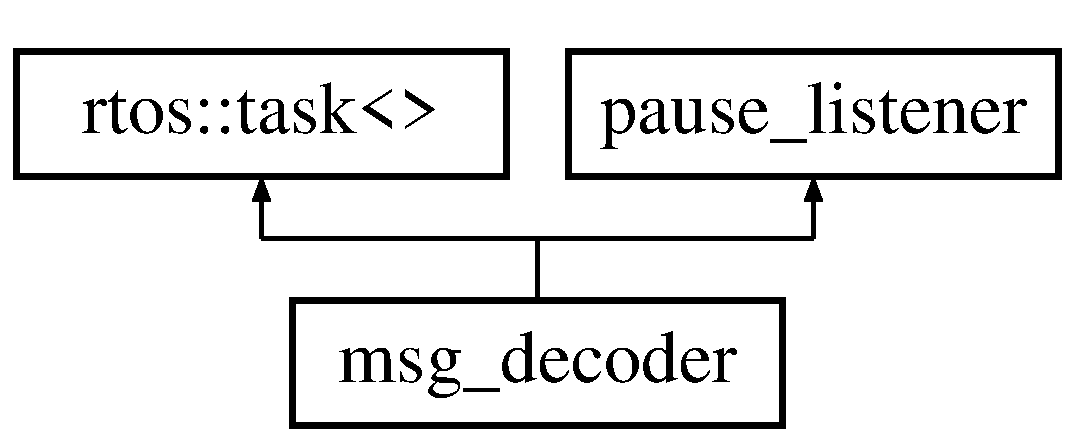
\includegraphics[height=2.000000cm]{classmsg__decoder}
\end{center}
\end{figure}
\subsection*{Public Member Functions}
\begin{DoxyCompactItemize}
\item 
\mbox{\Hypertarget{classmsg__decoder_ae9b18eff0ca3fc3d3c9248e4e38fd246}\label{classmsg__decoder_ae9b18eff0ca3fc3d3c9248e4e38fd246}} 
{\bfseries msg\+\_\+decoder} (const char $\ast$name, \mbox{\hyperlink{classmsg__listener}{msg\+\_\+listener}} \&listener)
\item 
\mbox{\Hypertarget{classmsg__decoder_a990f6ed2f479d61c8fbd0ceeba80a165}\label{classmsg__decoder_a990f6ed2f479d61c8fbd0ceeba80a165}} 
virtual void {\bfseries pause\+\_\+detected} (int pause\+\_\+length) override
\item 
\mbox{\Hypertarget{classmsg__decoder_a346301483ec894f687c93227d09a00a6}\label{classmsg__decoder_a346301483ec894f687c93227d09a00a6}} 
void {\bfseries print\+Byte} (uint8\+\_\+t byte)
\item 
\mbox{\Hypertarget{classmsg__decoder_af25ea64b8c252a82e879451c1fce6d24}\label{classmsg__decoder_af25ea64b8c252a82e879451c1fce6d24}} 
void {\bfseries print\+Bytes} (uint16\+\_\+t byte)
\item 
\mbox{\Hypertarget{classmsg__decoder_a17ed2804e6ec965a054b53e54b257d30}\label{classmsg__decoder_a17ed2804e6ec965a054b53e54b257d30}} 
bool {\bfseries check} (unsigned int m)
\item 
\mbox{\Hypertarget{classmsg__decoder_a8954f1ed668d0428ab4191ba6013c659}\label{classmsg__decoder_a8954f1ed668d0428ab4191ba6013c659}} 
void {\bfseries main} () override
\end{DoxyCompactItemize}


The documentation for this class was generated from the following file\+:\begin{DoxyCompactItemize}
\item 
C\+:/ti-\/software/thema\+\_\+opdracht\+\_\+lasergame/\+I\+R\+\_\+receive/msg\+\_\+decoder.\+hpp\end{DoxyCompactItemize}

\hypertarget{classmsg__listener}{}\section{msg\+\_\+listener Class Reference}
\label{classmsg__listener}\index{msg\+\_\+listener@{msg\+\_\+listener}}
Inheritance diagram for msg\+\_\+listener\+:\begin{figure}[H]
\begin{center}
\leavevmode
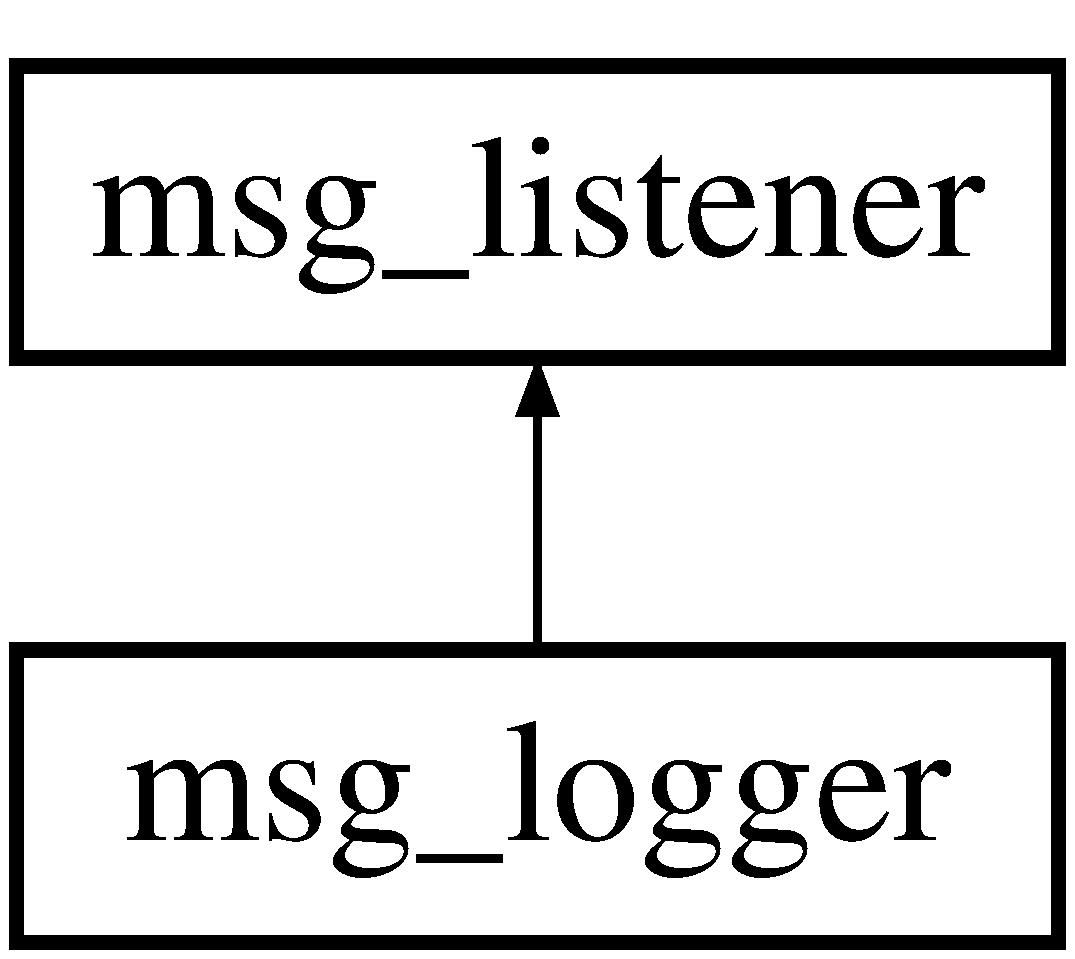
\includegraphics[height=2.000000cm]{classmsg__listener}
\end{center}
\end{figure}
\subsection*{Public Member Functions}
\begin{DoxyCompactItemize}
\item 
\mbox{\Hypertarget{classmsg__listener_ab82f5182543d7e9f2579e5d6f47cc3b9}\label{classmsg__listener_ab82f5182543d7e9f2579e5d6f47cc3b9}} 
virtual void {\bfseries msg\+\_\+received} (const \mbox{\hyperlink{structir__msg}{ir\+\_\+msg}} \&msg)=0
\end{DoxyCompactItemize}


The documentation for this class was generated from the following file\+:\begin{DoxyCompactItemize}
\item 
C\+:/ti-\/software/thema\+\_\+opdracht\+\_\+lasergame/\+I\+R\+\_\+receive/msg\+\_\+listener.\+hpp\end{DoxyCompactItemize}

\hypertarget{classmsg__logger}{}\section{msg\+\_\+logger Class Reference}
\label{classmsg__logger}\index{msg\+\_\+logger@{msg\+\_\+logger}}
Inheritance diagram for msg\+\_\+logger\+:\begin{figure}[H]
\begin{center}
\leavevmode
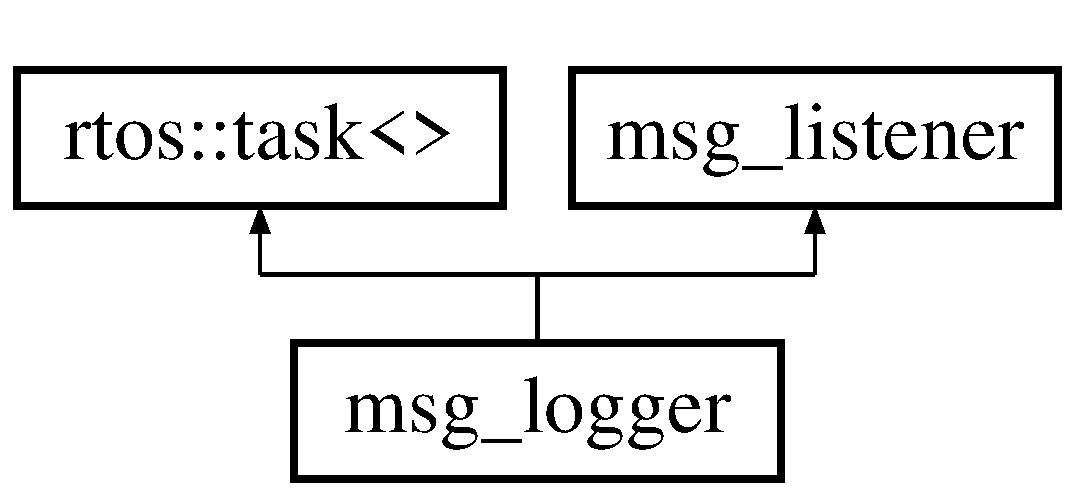
\includegraphics[height=2.000000cm]{classmsg__logger}
\end{center}
\end{figure}
\subsection*{Public Member Functions}
\begin{DoxyCompactItemize}
\item 
\mbox{\Hypertarget{classmsg__logger_a3ae26749c728559cb363631a7810f014}\label{classmsg__logger_a3ae26749c728559cb363631a7810f014}} 
{\bfseries msg\+\_\+logger} (const char $\ast$name)
\item 
\mbox{\Hypertarget{classmsg__logger_a1d6398b619717cccc6e125a660d6ad30}\label{classmsg__logger_a1d6398b619717cccc6e125a660d6ad30}} 
virtual void {\bfseries msg\+\_\+received} (const \mbox{\hyperlink{structir__msg}{ir\+\_\+msg}} \&msg) override
\item 
\mbox{\Hypertarget{classmsg__logger_ac674c87e969c7a22f483c809bf868460}\label{classmsg__logger_ac674c87e969c7a22f483c809bf868460}} 
void {\bfseries main} () override
\end{DoxyCompactItemize}


The documentation for this class was generated from the following file\+:\begin{DoxyCompactItemize}
\item 
C\+:/ti-\/software/thema\+\_\+opdracht\+\_\+lasergame/\+I\+R\+\_\+receive/msg\+\_\+logger.\+hpp\end{DoxyCompactItemize}

\hypertarget{class_msg_decoder}{}\section{Msg\+Decoder Class Reference}
\label{class_msg_decoder}\index{Msg\+Decoder@{Msg\+Decoder}}


This class decodes the incoming message and sends it to another class.  




{\ttfamily \#include $<$Msg\+Decoder.\+hpp$>$}

Inheritance diagram for Msg\+Decoder\+:\begin{figure}[H]
\begin{center}
\leavevmode
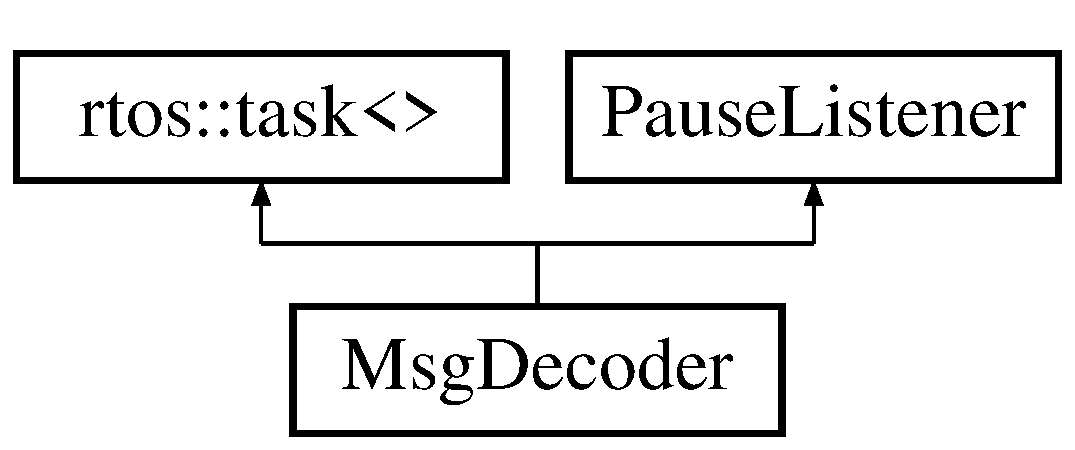
\includegraphics[height=2.000000cm]{class_msg_decoder}
\end{center}
\end{figure}
\subsection*{Public Member Functions}
\begin{DoxyCompactItemize}
\item 
\mbox{\hyperlink{class_msg_decoder_adc14f0f7ba3c05ef362502b54ffa2970}{Msg\+Decoder}} (const char $\ast$name, int priority, \mbox{\hyperlink{class_msg_listener}{Msg\+Listener}} \&listener)
\begin{DoxyCompactList}\small\item\em This is the constructor for the messagedecoder. \end{DoxyCompactList}\item 
virtual void \mbox{\hyperlink{class_msg_decoder_ac83f1179595fbd34295668baf17385fc}{pause\+Detected}} (int pause\+\_\+length) override
\begin{DoxyCompactList}\small\item\em This function overwrites the virtual pause\+Detected function. \end{DoxyCompactList}\item 
bool \mbox{\hyperlink{class_msg_decoder_a8dd1cc50baab5555661a9a9af7f3949f}{check}} (unsigned int m)
\begin{DoxyCompactList}\small\item\em This function checks if the message is valid. \end{DoxyCompactList}\item 
void \mbox{\hyperlink{class_msg_decoder_a0bf9b7579b386b8c9e18a9c606e80604}{main}} () override
\begin{DoxyCompactList}\small\item\em This function contains the state machine. \end{DoxyCompactList}\end{DoxyCompactItemize}


\subsection{Detailed Description}
This class decodes the incoming message and sends it to another class. 

\subsection{Constructor \& Destructor Documentation}
\mbox{\Hypertarget{class_msg_decoder_adc14f0f7ba3c05ef362502b54ffa2970}\label{class_msg_decoder_adc14f0f7ba3c05ef362502b54ffa2970}} 
\index{Msg\+Decoder@{Msg\+Decoder}!Msg\+Decoder@{Msg\+Decoder}}
\index{Msg\+Decoder@{Msg\+Decoder}!Msg\+Decoder@{Msg\+Decoder}}
\subsubsection{\texorpdfstring{Msg\+Decoder()}{MsgDecoder()}}
{\footnotesize\ttfamily Msg\+Decoder\+::\+Msg\+Decoder (\begin{DoxyParamCaption}\item[{const char $\ast$}]{name,  }\item[{int}]{priority,  }\item[{\mbox{\hyperlink{class_msg_listener}{Msg\+Listener}} \&}]{listener }\end{DoxyParamCaption})\hspace{0.3cm}{\ttfamily [inline]}}



This is the constructor for the messagedecoder. 

The constructor expects a listener to send the decoded message to. 

\subsection{Member Function Documentation}
\mbox{\Hypertarget{class_msg_decoder_a8dd1cc50baab5555661a9a9af7f3949f}\label{class_msg_decoder_a8dd1cc50baab5555661a9a9af7f3949f}} 
\index{Msg\+Decoder@{Msg\+Decoder}!check@{check}}
\index{check@{check}!Msg\+Decoder@{Msg\+Decoder}}
\subsubsection{\texorpdfstring{check()}{check()}}
{\footnotesize\ttfamily bool Msg\+Decoder\+::check (\begin{DoxyParamCaption}\item[{unsigned int}]{m }\end{DoxyParamCaption})\hspace{0.3cm}{\ttfamily [inline]}}



This function checks if the message is valid. 

This function compares the xor bits with the with xor of the player and weapon bits. The function returns true if the message is valid and false if it is not. \mbox{\Hypertarget{class_msg_decoder_a0bf9b7579b386b8c9e18a9c606e80604}\label{class_msg_decoder_a0bf9b7579b386b8c9e18a9c606e80604}} 
\index{Msg\+Decoder@{Msg\+Decoder}!main@{main}}
\index{main@{main}!Msg\+Decoder@{Msg\+Decoder}}
\subsubsection{\texorpdfstring{main()}{main()}}
{\footnotesize\ttfamily void Msg\+Decoder\+::main (\begin{DoxyParamCaption}{ }\end{DoxyParamCaption})\hspace{0.3cm}{\ttfamily [inline]}, {\ttfamily [override]}}



This function contains the state machine. 

The functions contains two states. In the idle state it waits for a pause and checks if the pause is valid. In the message state it checks if the following pause is valid and inserts a 1 or a 0 in the message respectively. If 16 valid pauses are detected the message gets sent with the message\+Detected function and it returns to the idle state. \mbox{\Hypertarget{class_msg_decoder_ac83f1179595fbd34295668baf17385fc}\label{class_msg_decoder_ac83f1179595fbd34295668baf17385fc}} 
\index{Msg\+Decoder@{Msg\+Decoder}!pause\+Detected@{pause\+Detected}}
\index{pause\+Detected@{pause\+Detected}!Msg\+Decoder@{Msg\+Decoder}}
\subsubsection{\texorpdfstring{pause\+Detected()}{pauseDetected()}}
{\footnotesize\ttfamily virtual void Msg\+Decoder\+::pause\+Detected (\begin{DoxyParamCaption}\item[{int}]{pause\+\_\+length }\end{DoxyParamCaption})\hspace{0.3cm}{\ttfamily [inline]}, {\ttfamily [override]}, {\ttfamily [virtual]}}



This function overwrites the virtual pause\+Detected function. 

This function writes the parameter pause\+\_\+length into the channel pauses. 

Implements \mbox{\hyperlink{class_pause_listener_ad2a8cbca3aa46215a54b96bfc84cc78b}{Pause\+Listener}}.



The documentation for this class was generated from the following file\+:\begin{DoxyCompactItemize}
\item 
C\+:/ti-\/software/thema\+\_\+opdracht\+\_\+lasergame/\+Player/\mbox{\hyperlink{_msg_decoder_8hpp}{Msg\+Decoder.\+hpp}}\end{DoxyCompactItemize}

\hypertarget{class_msg_listener}{}\section{Msg\+Listener Class Reference}
\label{class_msg_listener}\index{Msg\+Listener@{Msg\+Listener}}


This class constains the virtual msg\+Received function.  




{\ttfamily \#include $<$Msg\+Listener.\+hpp$>$}

Inheritance diagram for Msg\+Listener\+:\begin{figure}[H]
\begin{center}
\leavevmode
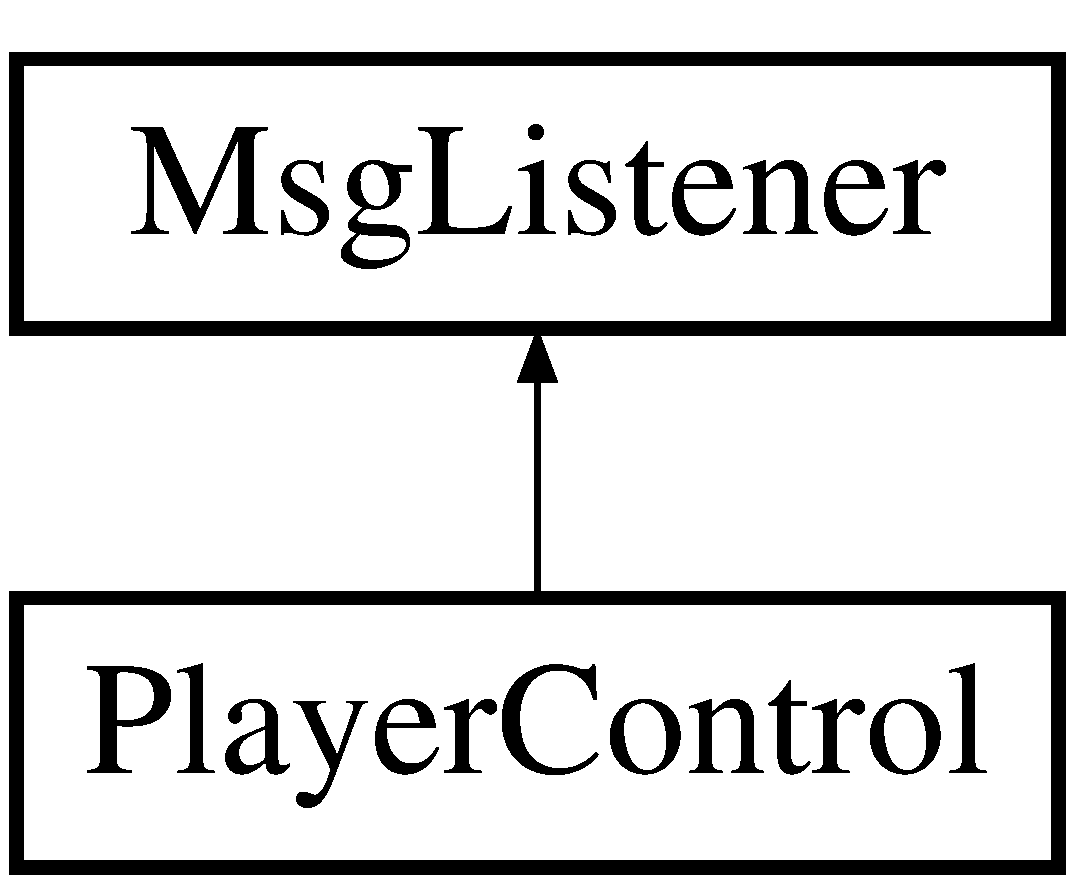
\includegraphics[height=2.000000cm]{class_msg_listener}
\end{center}
\end{figure}
\subsection*{Public Member Functions}
\begin{DoxyCompactItemize}
\item 
\mbox{\Hypertarget{class_msg_listener_a3bc48941e56b25199de434548513fd06}\label{class_msg_listener_a3bc48941e56b25199de434548513fd06}} 
virtual void \mbox{\hyperlink{class_msg_listener_a3bc48941e56b25199de434548513fd06}{msg\+Received}} (const \mbox{\hyperlink{structir__msg}{ir\+\_\+msg}} \&msg)=0
\begin{DoxyCompactList}\small\item\em This function gets called by the \mbox{\hyperlink{class_msg_decoder}{Msg\+Decoder}} and sends the message to the class that overwrites this function. \end{DoxyCompactList}\end{DoxyCompactItemize}


\subsection{Detailed Description}
This class constains the virtual msg\+Received function. 

The documentation for this class was generated from the following file\+:\begin{DoxyCompactItemize}
\item 
C\+:/ti-\/software/thema\+\_\+opdracht\+\_\+lasergame/\+Player/\mbox{\hyperlink{_msg_listener_8hpp}{Msg\+Listener.\+hpp}}\end{DoxyCompactItemize}

\hypertarget{classpause__detector}{}\section{pause\+\_\+detector Class Reference}
\label{classpause__detector}\index{pause\+\_\+detector@{pause\+\_\+detector}}
Inheritance diagram for pause\+\_\+detector\+:\begin{figure}[H]
\begin{center}
\leavevmode
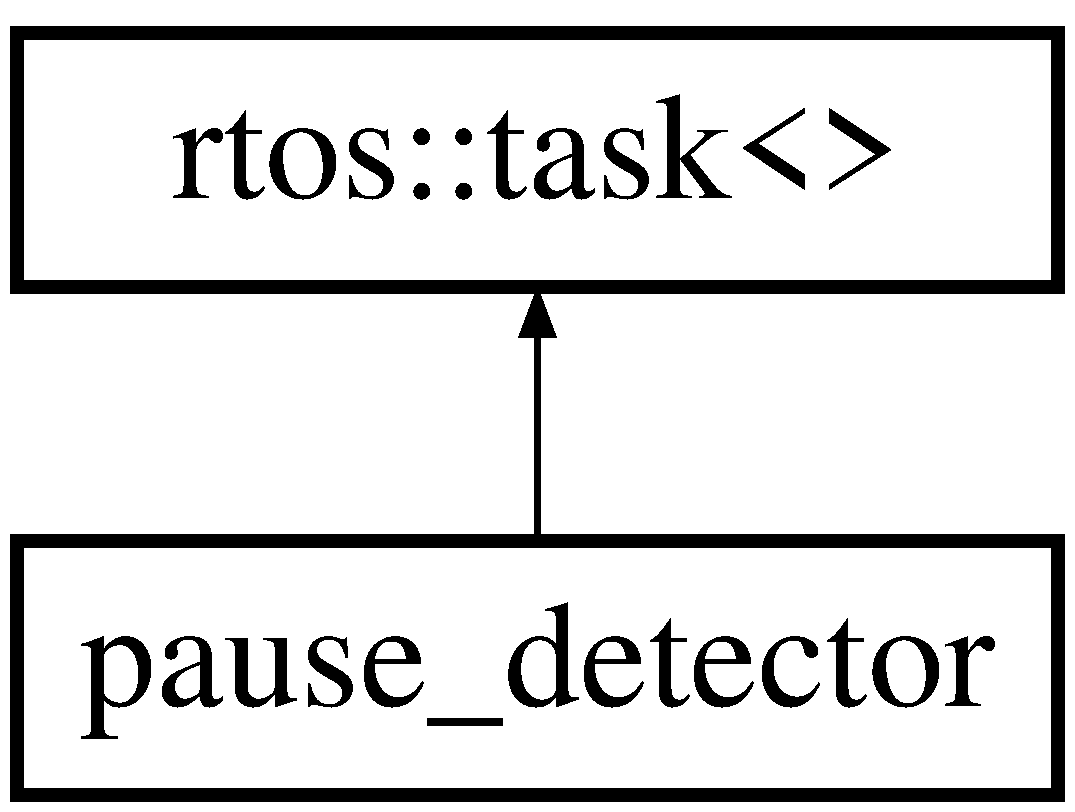
\includegraphics[height=2.000000cm]{classpause__detector}
\end{center}
\end{figure}
\subsection*{Public Member Functions}
\begin{DoxyCompactItemize}
\item 
\mbox{\Hypertarget{classpause__detector_a86b2fb4fd1032eb81517bc27ee9f6f2e}\label{classpause__detector_a86b2fb4fd1032eb81517bc27ee9f6f2e}} 
{\bfseries pause\+\_\+detector} (const char $\ast$name, hwlib\+::pin\+\_\+in \&irp, \mbox{\hyperlink{classpause__listener}{pause\+\_\+listener}} \&listener)
\item 
\mbox{\Hypertarget{classpause__detector_ac2d43c7fd2489b622359de11bfdc1cc2}\label{classpause__detector_ac2d43c7fd2489b622359de11bfdc1cc2}} 
void {\bfseries main} () override
\end{DoxyCompactItemize}


The documentation for this class was generated from the following file\+:\begin{DoxyCompactItemize}
\item 
C\+:/ti-\/software/thema\+\_\+opdracht\+\_\+lasergame/\+I\+R\+\_\+receive/pause\+\_\+detector.\+hpp\end{DoxyCompactItemize}

\hypertarget{classpause__listener}{}\section{pause\+\_\+listener Class Reference}
\label{classpause__listener}\index{pause\+\_\+listener@{pause\+\_\+listener}}
Inheritance diagram for pause\+\_\+listener\+:\begin{figure}[H]
\begin{center}
\leavevmode
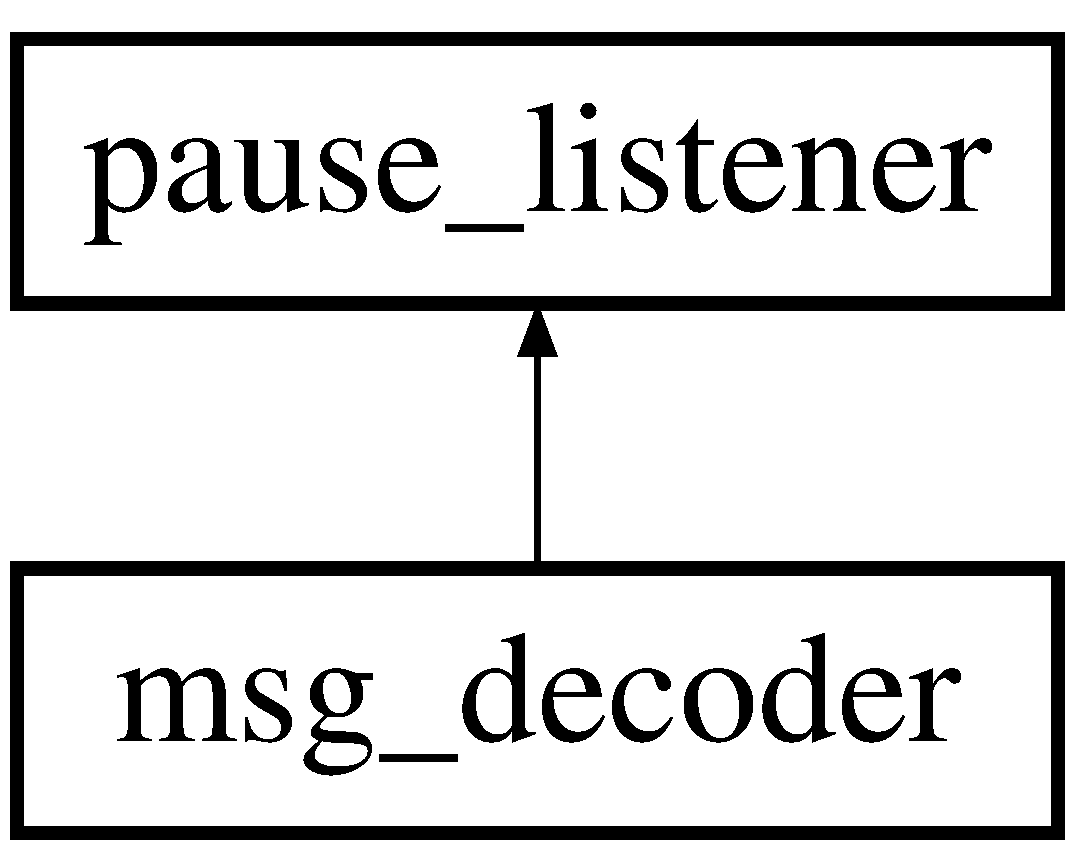
\includegraphics[height=2.000000cm]{classpause__listener}
\end{center}
\end{figure}
\subsection*{Public Member Functions}
\begin{DoxyCompactItemize}
\item 
\mbox{\Hypertarget{classpause__listener_a8c028680b7e4b26b7258417e0fb4cfca}\label{classpause__listener_a8c028680b7e4b26b7258417e0fb4cfca}} 
virtual void {\bfseries pause\+\_\+detected} (int pause\+\_\+length)=0
\end{DoxyCompactItemize}


The documentation for this class was generated from the following file\+:\begin{DoxyCompactItemize}
\item 
C\+:/ti-\/software/thema\+\_\+opdracht\+\_\+lasergame/\+I\+R\+\_\+receive/pause\+\_\+listener.\+hpp\end{DoxyCompactItemize}

\hypertarget{class_pause_detector}{}\section{Pause\+Detector Class Reference}
\label{class_pause_detector}\index{Pause\+Detector@{Pause\+Detector}}


This class detects the pauses in a IR signal and sends them to another class.  




{\ttfamily \#include $<$Pause\+Detector.\+hpp$>$}

Inheritance diagram for Pause\+Detector\+:\begin{figure}[H]
\begin{center}
\leavevmode
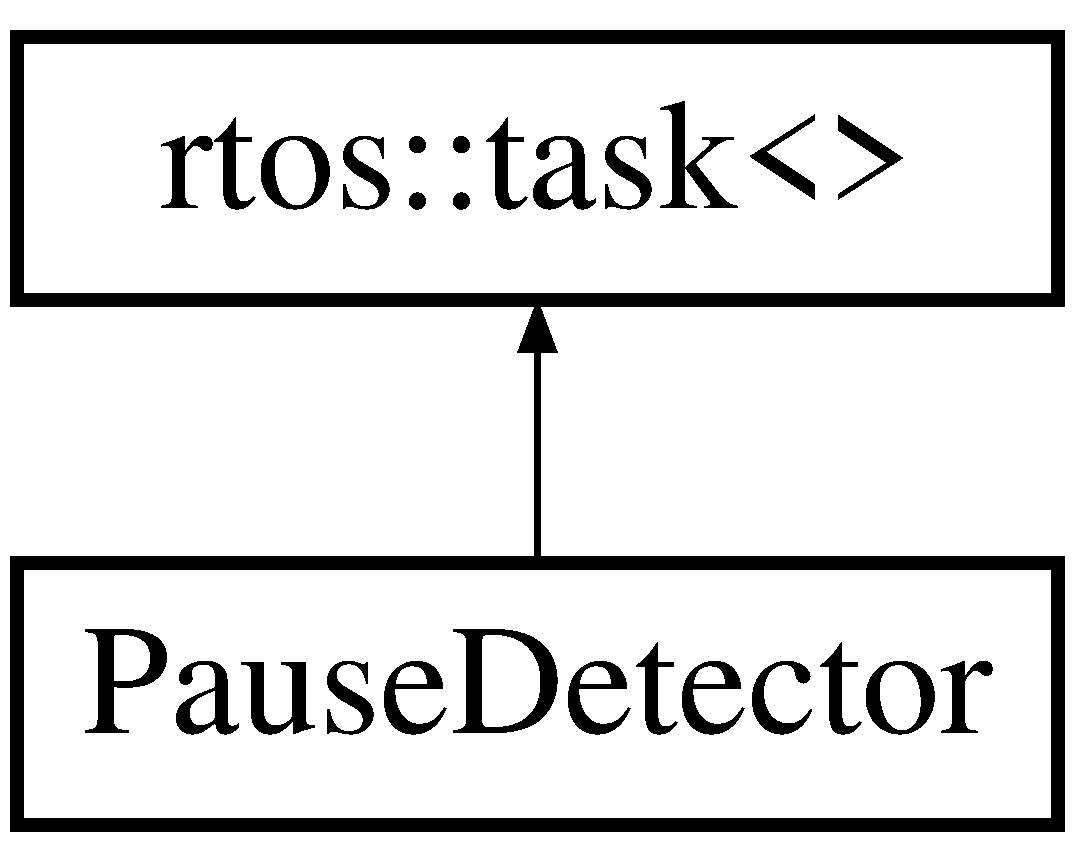
\includegraphics[height=2.000000cm]{class_pause_detector}
\end{center}
\end{figure}
\subsection*{Public Member Functions}
\begin{DoxyCompactItemize}
\item 
\mbox{\hyperlink{class_pause_detector_a89abb61f172dcdcdda2ab5ce3792983f}{Pause\+Detector}} (const char $\ast$name, int priority, hwlib\+::pin\+\_\+in \&irp, \mbox{\hyperlink{class_pause_listener}{Pause\+Listener}} \&listener)
\begin{DoxyCompactList}\small\item\em This is the constructor for the pause\+Detector. \end{DoxyCompactList}\item 
void \mbox{\hyperlink{class_pause_detector_a0ee4661673d1e5604877903c5d2cb35e}{main}} () override
\begin{DoxyCompactList}\small\item\em This function contains the state machine. \end{DoxyCompactList}\end{DoxyCompactItemize}


\subsection{Detailed Description}
This class detects the pauses in a IR signal and sends them to another class. 

\subsection{Constructor \& Destructor Documentation}
\mbox{\Hypertarget{class_pause_detector_a89abb61f172dcdcdda2ab5ce3792983f}\label{class_pause_detector_a89abb61f172dcdcdda2ab5ce3792983f}} 
\index{Pause\+Detector@{Pause\+Detector}!Pause\+Detector@{Pause\+Detector}}
\index{Pause\+Detector@{Pause\+Detector}!Pause\+Detector@{Pause\+Detector}}
\subsubsection{\texorpdfstring{Pause\+Detector()}{PauseDetector()}}
{\footnotesize\ttfamily Pause\+Detector\+::\+Pause\+Detector (\begin{DoxyParamCaption}\item[{const char $\ast$}]{name,  }\item[{int}]{priority,  }\item[{hwlib\+::pin\+\_\+in \&}]{irp,  }\item[{\mbox{\hyperlink{class_pause_listener}{Pause\+Listener}} \&}]{listener }\end{DoxyParamCaption})\hspace{0.3cm}{\ttfamily [inline]}}



This is the constructor for the pause\+Detector. 

The constructor expects a listener to send the detected messages to. 

\subsection{Member Function Documentation}
\mbox{\Hypertarget{class_pause_detector_a0ee4661673d1e5604877903c5d2cb35e}\label{class_pause_detector_a0ee4661673d1e5604877903c5d2cb35e}} 
\index{Pause\+Detector@{Pause\+Detector}!main@{main}}
\index{main@{main}!Pause\+Detector@{Pause\+Detector}}
\subsubsection{\texorpdfstring{main()}{main()}}
{\footnotesize\ttfamily void Pause\+Detector\+::main (\begin{DoxyParamCaption}{ }\end{DoxyParamCaption})\hspace{0.3cm}{\ttfamily [inline]}, {\ttfamily [override]}}



This function contains the state machine. 

The state machine consists of two states. The idle state waits every 100 us and checks if a pause is detected. If the pause ends it gets sent to the listener class and switches to the signal state. When a new pause starts the state switches to idle. 

The documentation for this class was generated from the following file\+:\begin{DoxyCompactItemize}
\item 
C\+:/ti-\/software/thema\+\_\+opdracht\+\_\+lasergame/\+Player/\mbox{\hyperlink{_pause_detector_8hpp}{Pause\+Detector.\+hpp}}\end{DoxyCompactItemize}

\hypertarget{class_pause_listener}{}\section{Pause\+Listener Class Reference}
\label{class_pause_listener}\index{Pause\+Listener@{Pause\+Listener}}


This class contains the virtual function pause\+Detected.  




{\ttfamily \#include $<$Pause\+Listener.\+hpp$>$}

Inheritance diagram for Pause\+Listener\+:\begin{figure}[H]
\begin{center}
\leavevmode
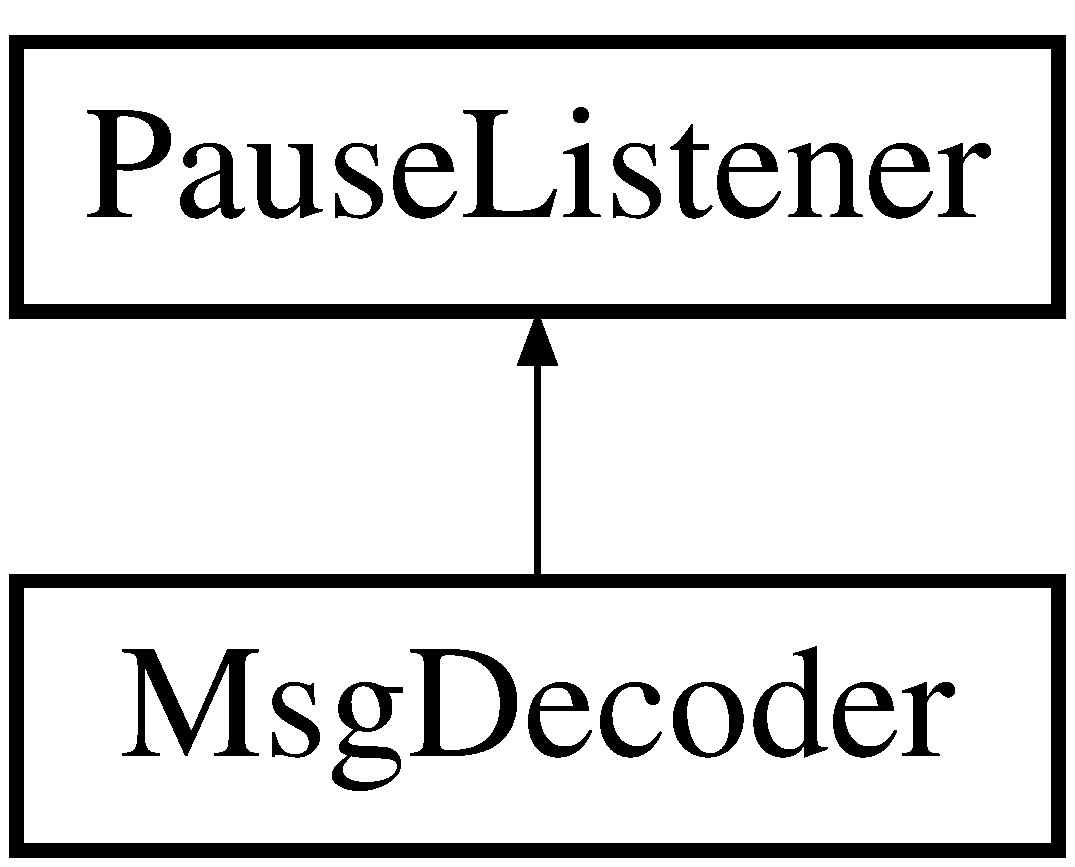
\includegraphics[height=2.000000cm]{class_pause_listener}
\end{center}
\end{figure}
\subsection*{Public Member Functions}
\begin{DoxyCompactItemize}
\item 
\mbox{\Hypertarget{class_pause_listener_ad2a8cbca3aa46215a54b96bfc84cc78b}\label{class_pause_listener_ad2a8cbca3aa46215a54b96bfc84cc78b}} 
virtual void \mbox{\hyperlink{class_pause_listener_ad2a8cbca3aa46215a54b96bfc84cc78b}{pause\+Detected}} (int pause\+\_\+length)=0
\begin{DoxyCompactList}\small\item\em The function gets called by the \mbox{\hyperlink{class_pause_detector}{Pause\+Detector}} and the pause gets sent to the class that overwrites the function. \end{DoxyCompactList}\end{DoxyCompactItemize}


\subsection{Detailed Description}
This class contains the virtual function pause\+Detected. 

The documentation for this class was generated from the following file\+:\begin{DoxyCompactItemize}
\item 
C\+:/ti-\/software/thema\+\_\+opdracht\+\_\+lasergame/\+Player/\mbox{\hyperlink{_pause_listener_8hpp}{Pause\+Listener.\+hpp}}\end{DoxyCompactItemize}

\hypertarget{class_player_control}{}\section{Player\+Control Class Reference}
\label{class_player_control}\index{Player\+Control@{Player\+Control}}


This class controls the player tasks.  




{\ttfamily \#include $<$Player\+Control.\+hpp$>$}

Inheritance diagram for Player\+Control\+:\begin{figure}[H]
\begin{center}
\leavevmode
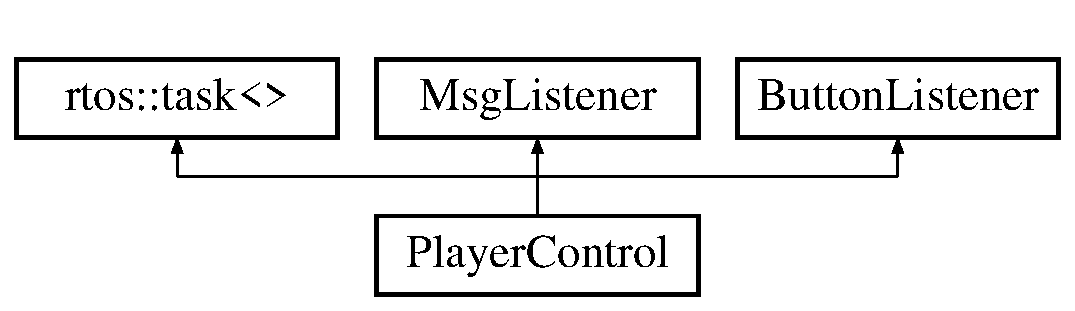
\includegraphics[height=2.000000cm]{class_player_control}
\end{center}
\end{figure}
\subsection*{Public Member Functions}
\begin{DoxyCompactItemize}
\item 
\mbox{\hyperlink{class_player_control_af026842ca91afba7f60da162f6fc527e}{Player\+Control}} (const char $\ast$name, int priority, \mbox{\hyperlink{class_shoot_control}{Shoot\+Control}} \&shoot\+\_\+control, \mbox{\hyperlink{class_display_control}{Display\+Control}} \&display\+\_\+control, \mbox{\hyperlink{class_buzzer_control}{Buzzer\+Control}} \&buzzer\+\_\+control, \mbox{\hyperlink{class_player_data}{Player\+Data}} \&player\+\_\+data, \mbox{\hyperlink{class_weapon}{Weapon}} \&weapon, \mbox{\hyperlink{class_game_logs}{Game\+Logs}} \&game\+\_\+logs, auto \&reload\+\_\+led, auto \&dead\+\_\+led)
\begin{DoxyCompactList}\small\item\em This is the constructor for the \mbox{\hyperlink{class_player_control}{Player\+Control}}. \end{DoxyCompactList}\item 
\mbox{\Hypertarget{class_player_control_af62429d7e940448496a196abf1bdc51f}\label{class_player_control_af62429d7e940448496a196abf1bdc51f}} 
void \mbox{\hyperlink{class_player_control_af62429d7e940448496a196abf1bdc51f}{set\+Player\+Number}} (uint8\+\_\+t player\+\_\+number)
\begin{DoxyCompactList}\small\item\em This function writes in the player\+\_\+number\+\_\+channel. \end{DoxyCompactList}\item 
\mbox{\Hypertarget{class_player_control_a73d535a1e16aadc234c6cd59e466305f}\label{class_player_control_a73d535a1e16aadc234c6cd59e466305f}} 
void \mbox{\hyperlink{class_player_control_a73d535a1e16aadc234c6cd59e466305f}{set\+Weapon}} (uint8\+\_\+t weapon\+\_\+number)
\begin{DoxyCompactList}\small\item\em This function writes in the player\+\_\+weapon\+\_\+channel. \end{DoxyCompactList}\item 
\mbox{\Hypertarget{class_player_control_a0d9fe3c384a800e4cd17cf15103b42c2}\label{class_player_control_a0d9fe3c384a800e4cd17cf15103b42c2}} 
virtual void \mbox{\hyperlink{class_player_control_a0d9fe3c384a800e4cd17cf15103b42c2}{msg\+Received}} (const \mbox{\hyperlink{structir__msg}{ir\+\_\+msg}} \&msg) override
\begin{DoxyCompactList}\small\item\em This function overwrites the msg\+Received function and writes the messsage in the msg\+\_\+channel. \end{DoxyCompactList}\item 
\mbox{\Hypertarget{class_player_control_a513d3c69e50d57af99b0dc14d86aa6c0}\label{class_player_control_a513d3c69e50d57af99b0dc14d86aa6c0}} 
virtual void \mbox{\hyperlink{class_player_control_a513d3c69e50d57af99b0dc14d86aa6c0}{button\+Pressed}} (unsigned int \&buttonnumber) override
\begin{DoxyCompactList}\small\item\em This function overwrites the button\+Pressed function and sets the flag depending on which button is pressed. \end{DoxyCompactList}\item 
void \mbox{\hyperlink{class_player_control_a9b3e136e412776977a658b232e7e9d6e}{main}} () override
\begin{DoxyCompactList}\small\item\em This function contains the state machine. \end{DoxyCompactList}\end{DoxyCompactItemize}


\subsection{Detailed Description}
This class controls the player tasks. 

\subsection{Constructor \& Destructor Documentation}
\mbox{\Hypertarget{class_player_control_af026842ca91afba7f60da162f6fc527e}\label{class_player_control_af026842ca91afba7f60da162f6fc527e}} 
\index{Player\+Control@{Player\+Control}!Player\+Control@{Player\+Control}}
\index{Player\+Control@{Player\+Control}!Player\+Control@{Player\+Control}}
\subsubsection{\texorpdfstring{Player\+Control()}{PlayerControl()}}
{\footnotesize\ttfamily Player\+Control\+::\+Player\+Control (\begin{DoxyParamCaption}\item[{const char $\ast$}]{name,  }\item[{int}]{priority,  }\item[{\mbox{\hyperlink{class_shoot_control}{Shoot\+Control}} \&}]{shoot\+\_\+control,  }\item[{\mbox{\hyperlink{class_display_control}{Display\+Control}} \&}]{display\+\_\+control,  }\item[{\mbox{\hyperlink{class_buzzer_control}{Buzzer\+Control}} \&}]{buzzer\+\_\+control,  }\item[{\mbox{\hyperlink{class_player_data}{Player\+Data}} \&}]{player\+\_\+data,  }\item[{\mbox{\hyperlink{class_weapon}{Weapon}} \&}]{weapon,  }\item[{\mbox{\hyperlink{class_game_logs}{Game\+Logs}} \&}]{game\+\_\+logs,  }\item[{auto \&}]{reload\+\_\+led,  }\item[{auto \&}]{dead\+\_\+led }\end{DoxyParamCaption})\hspace{0.3cm}{\ttfamily [inline]}}



This is the constructor for the \mbox{\hyperlink{class_player_control}{Player\+Control}}. 

The constructor expects shootcontrol, displaycontrol, buzzercontrol, playerdata, weapon, and gamelogs to send messages to or get data from. The constructor also expects two pins for the reload and dead leds. 

\subsection{Member Function Documentation}
\mbox{\Hypertarget{class_player_control_a9b3e136e412776977a658b232e7e9d6e}\label{class_player_control_a9b3e136e412776977a658b232e7e9d6e}} 
\index{Player\+Control@{Player\+Control}!main@{main}}
\index{main@{main}!Player\+Control@{Player\+Control}}
\subsubsection{\texorpdfstring{main()}{main()}}
{\footnotesize\ttfamily void Player\+Control\+::main (\begin{DoxyParamCaption}{ }\end{DoxyParamCaption})\hspace{0.3cm}{\ttfamily [inline]}, {\ttfamily [override]}}



This function contains the state machine. 

This function consists of 5 states. The state init\+\_\+game waits for the player\+\_\+number and player\+\_\+weapon from the keypad and a message from the msgdecoder. The message is used to set the game time and start the game. When the game starts the state becomes playing. The playing state consists of 3 states and starts with alive\+\_\+able\+\_\+to\+\_\+shoot. All three substates of playing wait for a game timer to end the game print the logs and transition back to the init state. The alive\+\_\+able\+\_\+to\+\_\+shoot state waits for the trigger or reload flag to set a timer and transition to the alive\+\_\+not\+\_\+able\+\_\+to\+\_\+shot state. It also waits for a message to check if the player gets hit. If the player dies the state transitions to the dead state. The alive\+\_\+not\+\_\+able\+\_\+to\+\_\+shoot state also waits for a message to check if the player gets hit. If the player dies the state transition to the dead state. If the timer set by the alive\+\_\+able\+\_\+to\+\_\+shoot state runs out the state transitions back to the alive\+\_\+able\+\_\+to\+\_\+shoot. The dead state resets the player health ammo and waits for the death timer. When the timer runs out the state transitions back to alive\+\_\+able\+\_\+to\+\_\+shoot. 

The documentation for this class was generated from the following file\+:\begin{DoxyCompactItemize}
\item 
C\+:/ti-\/software/thema\+\_\+opdracht\+\_\+lasergame/\+Player/\mbox{\hyperlink{_player_control_8hpp}{Player\+Control.\+hpp}}\end{DoxyCompactItemize}

\hypertarget{class_player_data}{}\section{Player\+Data Class Reference}
\label{class_player_data}\index{Player\+Data@{Player\+Data}}


This class contains all the playerdata.  




{\ttfamily \#include $<$Player\+Data.\+hpp$>$}

Inheritance diagram for Player\+Data\+:\begin{figure}[H]
\begin{center}
\leavevmode
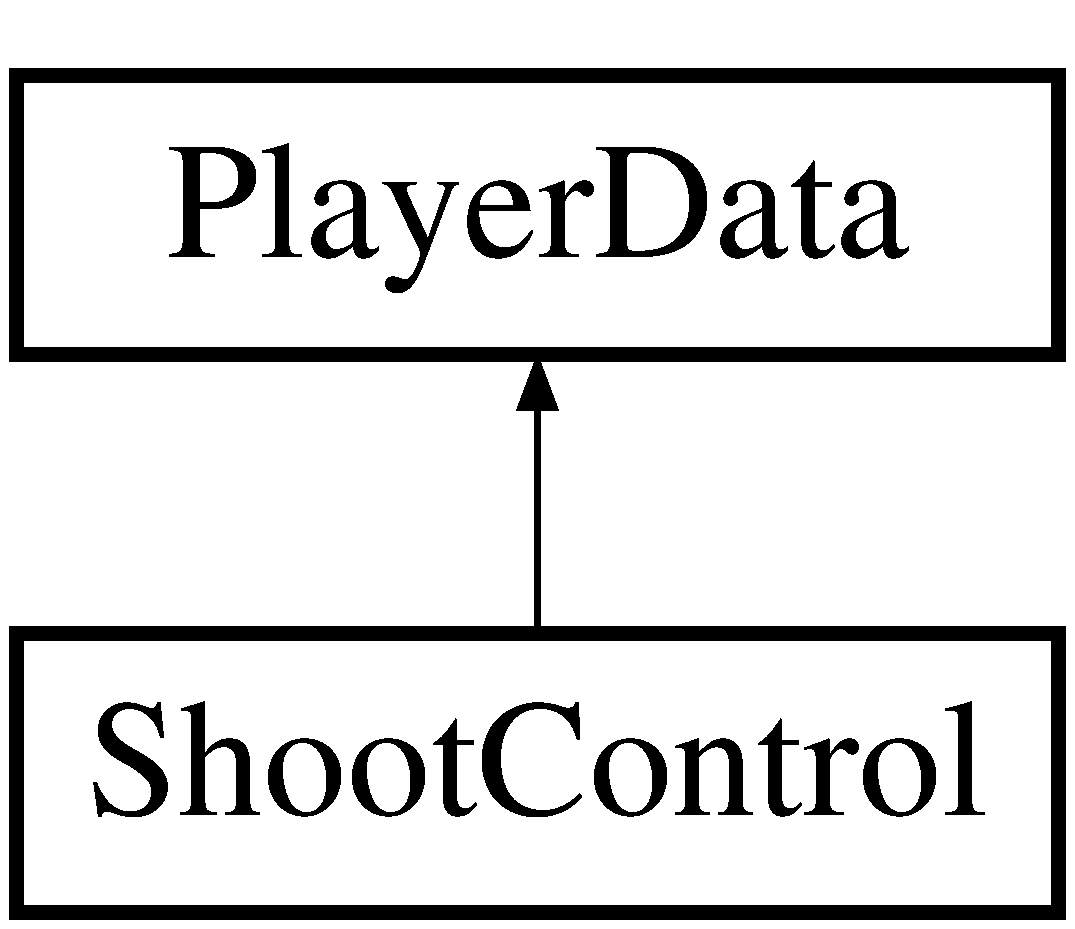
\includegraphics[height=2.000000cm]{class_player_data}
\end{center}
\end{figure}
\subsection*{Public Member Functions}
\begin{DoxyCompactItemize}
\item 
\mbox{\hyperlink{class_player_data_aaf3e4cbb80f8eb74f946fd858df68f19}{Player\+Data}} ()
\begin{DoxyCompactList}\small\item\em This is the constructor for the playerdata. \end{DoxyCompactList}\item 
\mbox{\Hypertarget{class_player_data_a9911cd97b9b1566c5add59ceb9bda3c5}\label{class_player_data_a9911cd97b9b1566c5add59ceb9bda3c5}} 
void \mbox{\hyperlink{class_player_data_a9911cd97b9b1566c5add59ceb9bda3c5}{set\+Player\+ID}} (uint8\+\_\+t player)
\begin{DoxyCompactList}\small\item\em This function sets the player\+ID. \end{DoxyCompactList}\item 
\mbox{\Hypertarget{class_player_data_a36f677fbe367f13a058a6f57509c7d3c}\label{class_player_data_a36f677fbe367f13a058a6f57509c7d3c}} 
void \mbox{\hyperlink{class_player_data_a36f677fbe367f13a058a6f57509c7d3c}{set\+Health}} (uint8\+\_\+t amount)
\begin{DoxyCompactList}\small\item\em This function sets the player health. \end{DoxyCompactList}\item 
\mbox{\Hypertarget{class_player_data_a5f19ad6aadf0a3432750f4277313bd9d}\label{class_player_data_a5f19ad6aadf0a3432750f4277313bd9d}} 
void \mbox{\hyperlink{class_player_data_a5f19ad6aadf0a3432750f4277313bd9d}{set\+Deaths}} (uint8\+\_\+t amount)
\begin{DoxyCompactList}\small\item\em This function sets the player deaths. \end{DoxyCompactList}\item 
\mbox{\Hypertarget{class_player_data_a941480a74b65933f0d82c891adcf0951}\label{class_player_data_a941480a74b65933f0d82c891adcf0951}} 
uint8\+\_\+t \mbox{\hyperlink{class_player_data_a941480a74b65933f0d82c891adcf0951}{get\+Player\+ID}} ()
\begin{DoxyCompactList}\small\item\em This function returns the player\+ID. \end{DoxyCompactList}\item 
\mbox{\Hypertarget{class_player_data_a21e83200b940047a4f90a9588569f0e8}\label{class_player_data_a21e83200b940047a4f90a9588569f0e8}} 
uint8\+\_\+t \mbox{\hyperlink{class_player_data_a21e83200b940047a4f90a9588569f0e8}{get\+Health}} ()
\begin{DoxyCompactList}\small\item\em This function returns the player health. \end{DoxyCompactList}\item 
\mbox{\Hypertarget{class_player_data_a9955efcfaa3b893ad984b78d5cf0f865}\label{class_player_data_a9955efcfaa3b893ad984b78d5cf0f865}} 
uint8\+\_\+t \mbox{\hyperlink{class_player_data_a9955efcfaa3b893ad984b78d5cf0f865}{get\+Max\+Health}} ()
\begin{DoxyCompactList}\small\item\em This function returns the maximum player health. \end{DoxyCompactList}\item 
\mbox{\Hypertarget{class_player_data_ac43afc297632fba65ae78e53c553780e}\label{class_player_data_ac43afc297632fba65ae78e53c553780e}} 
uint8\+\_\+t \mbox{\hyperlink{class_player_data_ac43afc297632fba65ae78e53c553780e}{get\+Deaths}} ()
\begin{DoxyCompactList}\small\item\em This function returns the player deaths. \end{DoxyCompactList}\item 
\mbox{\Hypertarget{class_player_data_aa6fa994c302c6aeaf1722bb7dd0b8cc0}\label{class_player_data_aa6fa994c302c6aeaf1722bb7dd0b8cc0}} 
uint8\+\_\+t \mbox{\hyperlink{class_player_data_aa6fa994c302c6aeaf1722bb7dd0b8cc0}{get\+Death\+Length}} ()
\begin{DoxyCompactList}\small\item\em This function returns the player death length. \end{DoxyCompactList}\end{DoxyCompactItemize}


\subsection{Detailed Description}
This class contains all the playerdata. 

\subsection{Constructor \& Destructor Documentation}
\mbox{\Hypertarget{class_player_data_aaf3e4cbb80f8eb74f946fd858df68f19}\label{class_player_data_aaf3e4cbb80f8eb74f946fd858df68f19}} 
\index{Player\+Data@{Player\+Data}!Player\+Data@{Player\+Data}}
\index{Player\+Data@{Player\+Data}!Player\+Data@{Player\+Data}}
\subsubsection{\texorpdfstring{Player\+Data()}{PlayerData()}}
{\footnotesize\ttfamily Player\+Data\+::\+Player\+Data (\begin{DoxyParamCaption}{ }\end{DoxyParamCaption})\hspace{0.3cm}{\ttfamily [inline]}}



This is the constructor for the playerdata. 

The constructor sets all the playerdata to default values. 

The documentation for this class was generated from the following file\+:\begin{DoxyCompactItemize}
\item 
C\+:/ti-\/software/thema\+\_\+opdracht\+\_\+lasergame/\+Player/\mbox{\hyperlink{_player_data_8hpp}{Player\+Data.\+hpp}}\end{DoxyCompactItemize}

\hypertarget{class_send_control}{}\section{Send\+Control Class Reference}
\label{class_send_control}\index{Send\+Control@{Send\+Control}}


This class is used to send the data.  




{\ttfamily \#include $<$Send\+Control.\+hpp$>$}

Inheritance diagram for Send\+Control\+:\begin{figure}[H]
\begin{center}
\leavevmode
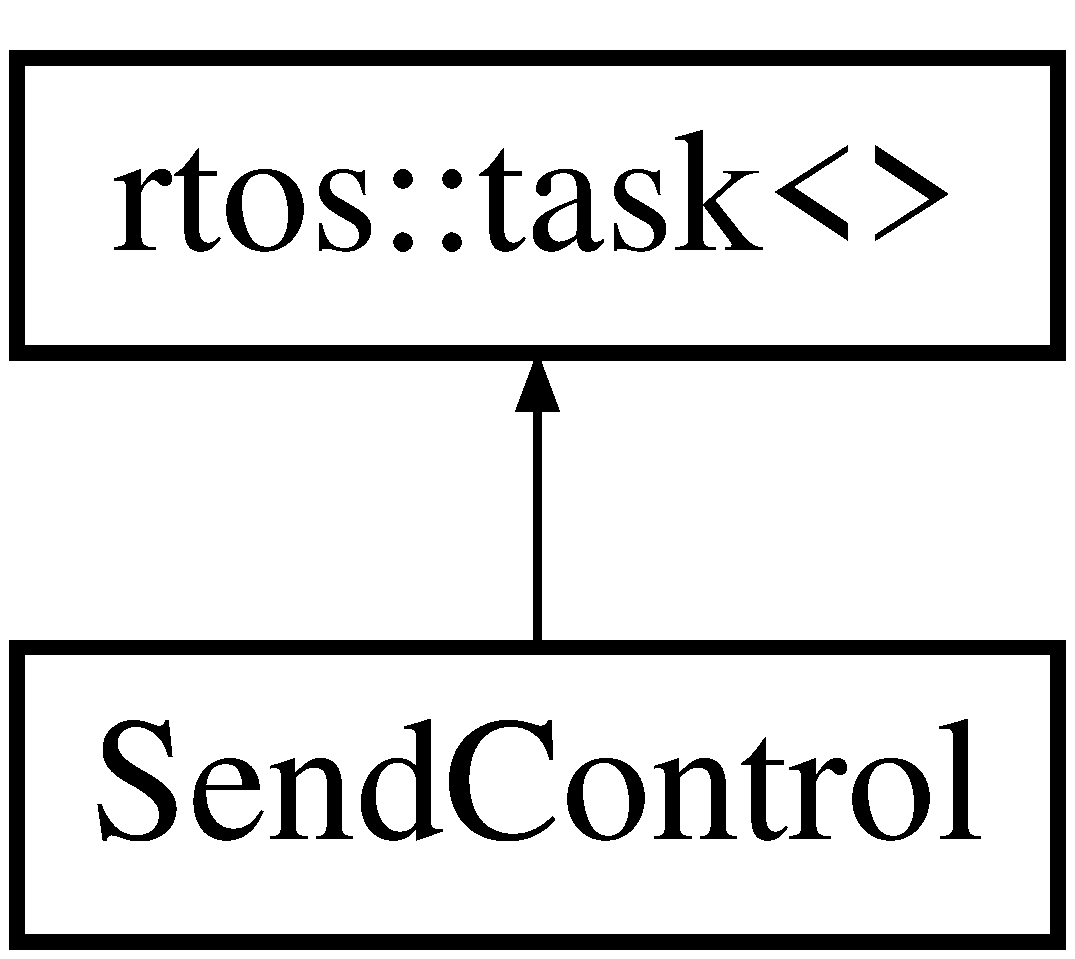
\includegraphics[height=2.000000cm]{class_send_control}
\end{center}
\end{figure}
\subsection*{Public Member Functions}
\begin{DoxyCompactItemize}
\item 
\mbox{\hyperlink{class_send_control_af666c41a0c262bf86bbb3009003b2c81}{Send\+Control}} (const char $\ast$name, int priority, \mbox{\hyperlink{class_i_r_control}{I\+R\+Control}} \&I\+R\+\_\+control)
\begin{DoxyCompactList}\small\item\em This is the constructer of send control. \end{DoxyCompactList}\item 
\mbox{\Hypertarget{class_send_control_a631b78165c258e5ee4bde7d0790385a0}\label{class_send_control_a631b78165c258e5ee4bde7d0790385a0}} 
void \mbox{\hyperlink{class_send_control_a631b78165c258e5ee4bde7d0790385a0}{send}} (uint8\+\_\+t data)
\begin{DoxyCompactList}\small\item\em This function writes the data in the send\+\_\+pool and sets the send\+\_\+flag. \end{DoxyCompactList}\item 
void \mbox{\hyperlink{class_send_control_aedec285713d090002e2848228cef2617}{main}} () override
\begin{DoxyCompactList}\small\item\em This is the state function for send control. \end{DoxyCompactList}\end{DoxyCompactItemize}


\subsection{Detailed Description}
This class is used to send the data. 

\subsection{Constructor \& Destructor Documentation}
\mbox{\Hypertarget{class_send_control_af666c41a0c262bf86bbb3009003b2c81}\label{class_send_control_af666c41a0c262bf86bbb3009003b2c81}} 
\index{Send\+Control@{Send\+Control}!Send\+Control@{Send\+Control}}
\index{Send\+Control@{Send\+Control}!Send\+Control@{Send\+Control}}
\subsubsection{\texorpdfstring{Send\+Control()}{SendControl()}}
{\footnotesize\ttfamily Send\+Control\+::\+Send\+Control (\begin{DoxyParamCaption}\item[{const char $\ast$}]{name,  }\item[{int}]{priority,  }\item[{\mbox{\hyperlink{class_i_r_control}{I\+R\+Control}} \&}]{I\+R\+\_\+control }\end{DoxyParamCaption})\hspace{0.3cm}{\ttfamily [inline]}}



This is the constructer of send control. 

The constructer wants IR control. 

\subsection{Member Function Documentation}
\mbox{\Hypertarget{class_send_control_aedec285713d090002e2848228cef2617}\label{class_send_control_aedec285713d090002e2848228cef2617}} 
\index{Send\+Control@{Send\+Control}!main@{main}}
\index{main@{main}!Send\+Control@{Send\+Control}}
\subsubsection{\texorpdfstring{main()}{main()}}
{\footnotesize\ttfamily void Send\+Control\+::main (\begin{DoxyParamCaption}{ }\end{DoxyParamCaption})\hspace{0.3cm}{\ttfamily [inline]}, {\ttfamily [override]}}



This is the state function for send control. 

This function has 1 state\+: I\+D\+LE. The function waits for the send\+\_\+flag and the call the set\+Send\+Data with as parameter an encoded game\+\_\+leader with send\+\_\+pool readed data. 

The documentation for this class was generated from the following file\+:\begin{DoxyCompactItemize}
\item 
C\+:/ti-\/software/thema\+\_\+opdracht\+\_\+lasergame/\+Gameleader/\mbox{\hyperlink{_send_control_8hpp}{Send\+Control.\+hpp}}\end{DoxyCompactItemize}

\hypertarget{class_shoot_control}{}\section{Shoot\+Control Class Reference}
\label{class_shoot_control}\index{Shoot\+Control@{Shoot\+Control}}


This class encodes and sends the message to be sent to the \mbox{\hyperlink{class_i_r_control}{I\+R\+Control}} class and controls the laser.  




{\ttfamily \#include $<$Shoot\+Control.\+hpp$>$}

Inheritance diagram for Shoot\+Control\+:\begin{figure}[H]
\begin{center}
\leavevmode
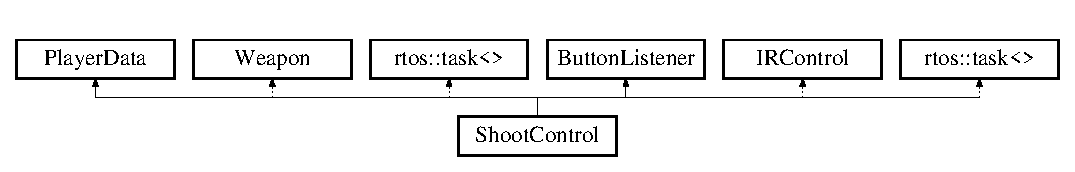
\includegraphics[height=2.000000cm]{class_shoot_control}
\end{center}
\end{figure}
\subsection*{Public Member Functions}
\begin{DoxyCompactItemize}
\item 
\mbox{\hyperlink{class_shoot_control_af9c21b16c798f217b2da762d569473cd}{Shoot\+Control}} (const char $\ast$name, int priority, \mbox{\hyperlink{class_i_r_control}{I\+R\+Control}} \&I\+R\+\_\+control, \mbox{\hyperlink{class_player_data}{Player\+Data}} \&player\+\_\+data, \mbox{\hyperlink{class_weapon}{Weapon}} \&weapon, hwlib\+::pin\+\_\+out \&laser\+\_\+pin)
\begin{DoxyCompactList}\small\item\em This is the constructor for the shoot\+Control. \end{DoxyCompactList}\item 
\mbox{\Hypertarget{class_shoot_control_a17f6db4ed8fb3a7195e03eb54b9c26f1}\label{class_shoot_control_a17f6db4ed8fb3a7195e03eb54b9c26f1}} 
void \mbox{\hyperlink{class_shoot_control_a17f6db4ed8fb3a7195e03eb54b9c26f1}{shoot}} ()
\begin{DoxyCompactList}\small\item\em This function sets the shoot\+\_\+flag.  This function is used to be called by another class. \end{DoxyCompactList}\item 
void \mbox{\hyperlink{class_shoot_control_afda9df061db3b34fdf9affed32f2c325}{main}} () override
\begin{DoxyCompactList}\small\item\em This function contains the state machine. \end{DoxyCompactList}\end{DoxyCompactItemize}


\subsection{Detailed Description}
This class encodes and sends the message to be sent to the \mbox{\hyperlink{class_i_r_control}{I\+R\+Control}} class and controls the laser. 

\subsection{Constructor \& Destructor Documentation}
\mbox{\Hypertarget{class_shoot_control_af9c21b16c798f217b2da762d569473cd}\label{class_shoot_control_af9c21b16c798f217b2da762d569473cd}} 
\index{Shoot\+Control@{Shoot\+Control}!Shoot\+Control@{Shoot\+Control}}
\index{Shoot\+Control@{Shoot\+Control}!Shoot\+Control@{Shoot\+Control}}
\subsubsection{\texorpdfstring{Shoot\+Control()}{ShootControl()}}
{\footnotesize\ttfamily Shoot\+Control\+::\+Shoot\+Control (\begin{DoxyParamCaption}\item[{const char $\ast$}]{name,  }\item[{int}]{priority,  }\item[{\mbox{\hyperlink{class_i_r_control}{I\+R\+Control}} \&}]{I\+R\+\_\+control,  }\item[{\mbox{\hyperlink{class_player_data}{Player\+Data}} \&}]{player\+\_\+data,  }\item[{\mbox{\hyperlink{class_weapon}{Weapon}} \&}]{weapon,  }\item[{hwlib\+::pin\+\_\+out \&}]{laser\+\_\+pin }\end{DoxyParamCaption})\hspace{0.3cm}{\ttfamily [inline]}}



This is the constructor for the shoot\+Control. 

The constructor expects the class \mbox{\hyperlink{class_i_r_control}{I\+R\+Control}} the enitities player\+\_\+data and weapon as well as a output pin for the laser. 

\subsection{Member Function Documentation}
\mbox{\Hypertarget{class_shoot_control_afda9df061db3b34fdf9affed32f2c325}\label{class_shoot_control_afda9df061db3b34fdf9affed32f2c325}} 
\index{Shoot\+Control@{Shoot\+Control}!main@{main}}
\index{main@{main}!Shoot\+Control@{Shoot\+Control}}
\subsubsection{\texorpdfstring{main()}{main()}}
{\footnotesize\ttfamily void Shoot\+Control\+::main (\begin{DoxyParamCaption}{ }\end{DoxyParamCaption})\hspace{0.3cm}{\ttfamily [inline]}, {\ttfamily [override]}}



This function contains the state machine. 

This function contains only one state called idle. The idle state waits for a shoot flag. When the shoot flag is set the laser turns on and the function set\+Send\+Data is called. After 100ms the laser is turned off and the state starts waiting for the shoot\+\_\+flag again. 

The documentation for this class was generated from the following file\+:\begin{DoxyCompactItemize}
\item 
C\+:/ti-\/software/thema\+\_\+opdracht\+\_\+lasergame/\+Player/\mbox{\hyperlink{_shoot_control_8hpp}{Shoot\+Control.\+hpp}}\end{DoxyCompactItemize}

\hypertarget{class_weapon}{}\section{Weapon Class Reference}
\label{class_weapon}\index{Weapon@{Weapon}}


This class contains the data of the weapon.  




{\ttfamily \#include $<$Weapon.\+hpp$>$}

Inheritance diagram for Weapon\+:\begin{figure}[H]
\begin{center}
\leavevmode
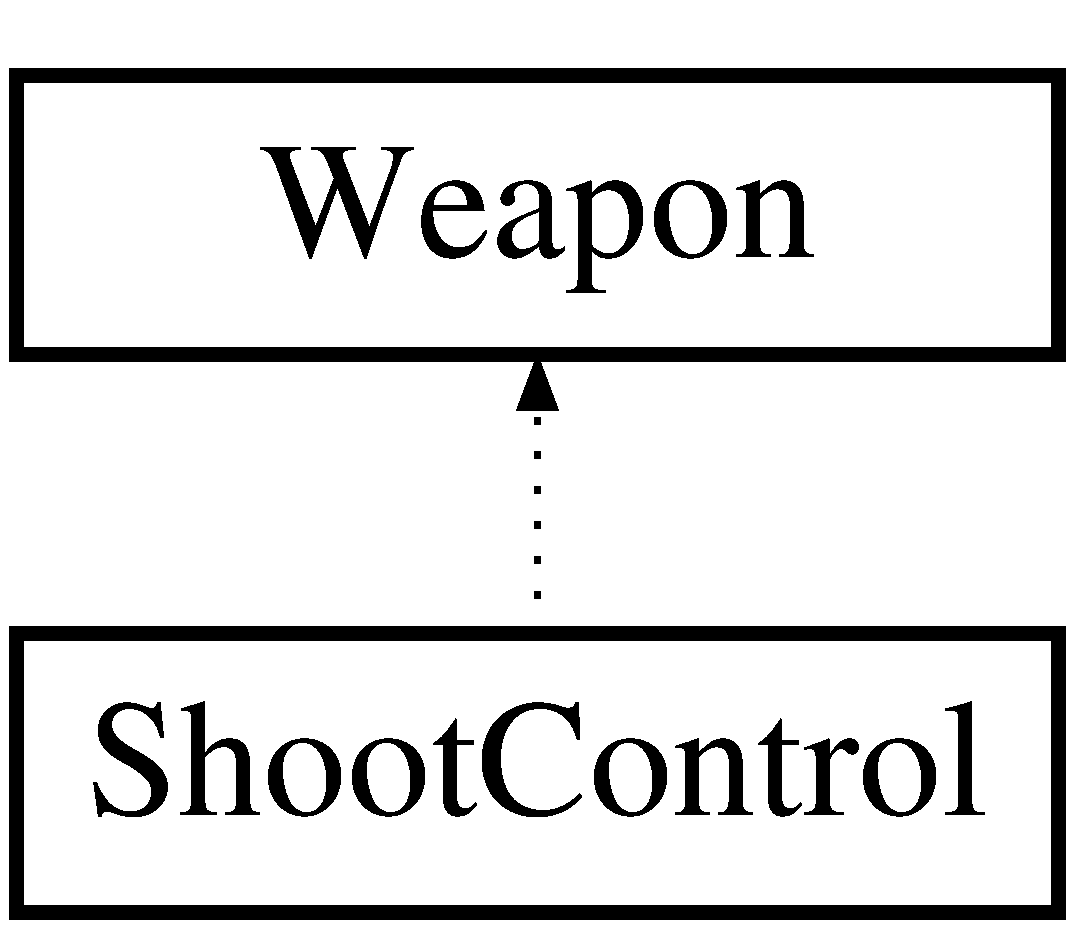
\includegraphics[height=2.000000cm]{class_weapon}
\end{center}
\end{figure}
\subsection*{Public Member Functions}
\begin{DoxyCompactItemize}
\item 
void \mbox{\hyperlink{class_weapon_a6d42418876685100d754e566c627aea7}{set\+Weapon}} (uint8\+\_\+t weapon)
\begin{DoxyCompactList}\small\item\em This is the constructor for the weapon class. \end{DoxyCompactList}\item 
\mbox{\Hypertarget{class_weapon_a1744536f5f55f6cf87d3e09d23b467c3}\label{class_weapon_a1744536f5f55f6cf87d3e09d23b467c3}} 
const char $\ast$ \mbox{\hyperlink{class_weapon_a1744536f5f55f6cf87d3e09d23b467c3}{get\+Weapon\+Name}} (uint8\+\_\+t weapon\+\_\+\+ID)
\begin{DoxyCompactList}\small\item\em This function returns the weapon name. \end{DoxyCompactList}\item 
\mbox{\Hypertarget{class_weapon_a2c20f2b180ea9445ced8fe76e181db63}\label{class_weapon_a2c20f2b180ea9445ced8fe76e181db63}} 
uint8\+\_\+t \mbox{\hyperlink{class_weapon_a2c20f2b180ea9445ced8fe76e181db63}{get\+Weapon\+Damage}} (uint8\+\_\+t weapon\+\_\+\+ID)
\begin{DoxyCompactList}\small\item\em This function returns the weapon damage. \end{DoxyCompactList}\item 
\mbox{\Hypertarget{class_weapon_ae290125f66f5c24272b6e708d078ef78}\label{class_weapon_ae290125f66f5c24272b6e708d078ef78}} 
uint8\+\_\+t \mbox{\hyperlink{class_weapon_ae290125f66f5c24272b6e708d078ef78}{get\+Weapon\+ID}} ()
\begin{DoxyCompactList}\small\item\em This function returns the weapon\+ID. \end{DoxyCompactList}\item 
\mbox{\Hypertarget{class_weapon_a40bcd96fc932869e50fd2e7287ec8d9c}\label{class_weapon_a40bcd96fc932869e50fd2e7287ec8d9c}} 
uint8\+\_\+t \mbox{\hyperlink{class_weapon_a40bcd96fc932869e50fd2e7287ec8d9c}{get\+Ammo}} ()
\begin{DoxyCompactList}\small\item\em This function returns the ammo of the weapon. \end{DoxyCompactList}\item 
\mbox{\Hypertarget{class_weapon_a32fb116e169af265f52b4f51e955f44f}\label{class_weapon_a32fb116e169af265f52b4f51e955f44f}} 
uint8\+\_\+t \mbox{\hyperlink{class_weapon_a32fb116e169af265f52b4f51e955f44f}{get\+Max\+Ammo}} ()
\begin{DoxyCompactList}\small\item\em This function returns the maximum ammo of the weapon. \end{DoxyCompactList}\item 
\mbox{\Hypertarget{class_weapon_aee03c3f7faeb4ac9e29dd72a1821d7fe}\label{class_weapon_aee03c3f7faeb4ac9e29dd72a1821d7fe}} 
uint8\+\_\+t \mbox{\hyperlink{class_weapon_aee03c3f7faeb4ac9e29dd72a1821d7fe}{get\+Shot\+Delay}} ()
\begin{DoxyCompactList}\small\item\em This function returns the shot delay of the weapon. \end{DoxyCompactList}\item 
\mbox{\Hypertarget{class_weapon_a25ab6dd12d10b3b64a78b775c3905b7a}\label{class_weapon_a25ab6dd12d10b3b64a78b775c3905b7a}} 
uint8\+\_\+t \mbox{\hyperlink{class_weapon_a25ab6dd12d10b3b64a78b775c3905b7a}{get\+Reload\+Time}} ()
\begin{DoxyCompactList}\small\item\em This function returns the reload time of the weapon. \end{DoxyCompactList}\item 
\mbox{\Hypertarget{class_weapon_a65871b565297b49dfdb5dcc00555a0b3}\label{class_weapon_a65871b565297b49dfdb5dcc00555a0b3}} 
void \mbox{\hyperlink{class_weapon_a65871b565297b49dfdb5dcc00555a0b3}{set\+Ammo}} (uint8\+\_\+t amount)
\begin{DoxyCompactList}\small\item\em This function sets the ammo for the weapon. \end{DoxyCompactList}\end{DoxyCompactItemize}


\subsection{Detailed Description}
This class contains the data of the weapon. 

\subsection{Member Function Documentation}
\mbox{\Hypertarget{class_weapon_a6d42418876685100d754e566c627aea7}\label{class_weapon_a6d42418876685100d754e566c627aea7}} 
\index{Weapon@{Weapon}!set\+Weapon@{set\+Weapon}}
\index{set\+Weapon@{set\+Weapon}!Weapon@{Weapon}}
\subsubsection{\texorpdfstring{set\+Weapon()}{setWeapon()}}
{\footnotesize\ttfamily void Weapon\+::set\+Weapon (\begin{DoxyParamCaption}\item[{uint8\+\_\+t}]{weapon }\end{DoxyParamCaption})\hspace{0.3cm}{\ttfamily [inline]}}



This is the constructor for the weapon class. 

The constructor sets all the weapon stats based on the number entered in the constructor. 

The documentation for this class was generated from the following file\+:\begin{DoxyCompactItemize}
\item 
C\+:/ti-\/software/thema\+\_\+opdracht\+\_\+lasergame/\+Player/\mbox{\hyperlink{_weapon_8hpp}{Weapon.\+hpp}}\end{DoxyCompactItemize}

\chapter{File Documentation}
\hypertarget{_gameleader_2_buzzer_control_8hpp}{}\section{C\+:/ti-\/software/thema\+\_\+opdracht\+\_\+lasergame/\+Gameleader/\+Buzzer\+Control.hpp File Reference}
\label{_gameleader_2_buzzer_control_8hpp}\index{C\+:/ti-\/software/thema\+\_\+opdracht\+\_\+lasergame/\+Gameleader/\+Buzzer\+Control.\+hpp@{C\+:/ti-\/software/thema\+\_\+opdracht\+\_\+lasergame/\+Gameleader/\+Buzzer\+Control.\+hpp}}
{\ttfamily \#include \char`\"{}hwlib.\+hpp\char`\"{}}\newline
{\ttfamily \#include \char`\"{}rtos.\+hpp\char`\"{}}\newline
\subsection*{Classes}
\begin{DoxyCompactItemize}
\item 
class \mbox{\hyperlink{class_buzzer_control}{Buzzer\+Control}}
\begin{DoxyCompactList}\small\item\em This class is used to control the buzzer. \end{DoxyCompactList}\end{DoxyCompactItemize}

\hypertarget{_player_2_buzzer_control_8hpp}{}\section{C\+:/ti-\/software/thema\+\_\+opdracht\+\_\+lasergame/\+Player/\+Buzzer\+Control.hpp File Reference}
\label{_player_2_buzzer_control_8hpp}\index{C\+:/ti-\/software/thema\+\_\+opdracht\+\_\+lasergame/\+Player/\+Buzzer\+Control.\+hpp@{C\+:/ti-\/software/thema\+\_\+opdracht\+\_\+lasergame/\+Player/\+Buzzer\+Control.\+hpp}}
{\ttfamily \#include \char`\"{}hwlib.\+hpp\char`\"{}}\newline
{\ttfamily \#include \char`\"{}rtos.\+hpp\char`\"{}}\newline
\subsection*{Classes}
\begin{DoxyCompactItemize}
\item 
class \mbox{\hyperlink{class_buzzer_control}{Buzzer\+Control}}
\begin{DoxyCompactList}\small\item\em This class is used to control the buzzer. \end{DoxyCompactList}\end{DoxyCompactItemize}

\hypertarget{_gameleader_2_display_control_8hpp}{}\section{C\+:/ti-\/software/thema\+\_\+opdracht\+\_\+lasergame/\+Gameleader/\+Display\+Control.hpp File Reference}
\label{_gameleader_2_display_control_8hpp}\index{C\+:/ti-\/software/thema\+\_\+opdracht\+\_\+lasergame/\+Gameleader/\+Display\+Control.\+hpp@{C\+:/ti-\/software/thema\+\_\+opdracht\+\_\+lasergame/\+Gameleader/\+Display\+Control.\+hpp}}
{\ttfamily \#include \char`\"{}hwlib.\+hpp\char`\"{}}\newline
{\ttfamily \#include \char`\"{}rtos.\+hpp\char`\"{}}\newline
\subsection*{Classes}
\begin{DoxyCompactItemize}
\item 
class \mbox{\hyperlink{class_display_control}{Display\+Control}}
\begin{DoxyCompactList}\small\item\em This class is used to show the command value on the screen. \end{DoxyCompactList}\end{DoxyCompactItemize}

\hypertarget{_player_2_display_control_8hpp}{}\section{C\+:/ti-\/software/thema\+\_\+opdracht\+\_\+lasergame/\+Player/\+Display\+Control.hpp File Reference}
\label{_player_2_display_control_8hpp}\index{C\+:/ti-\/software/thema\+\_\+opdracht\+\_\+lasergame/\+Player/\+Display\+Control.\+hpp@{C\+:/ti-\/software/thema\+\_\+opdracht\+\_\+lasergame/\+Player/\+Display\+Control.\+hpp}}
{\ttfamily \#include \char`\"{}hwlib.\+hpp\char`\"{}}\newline
{\ttfamily \#include \char`\"{}rtos.\+hpp\char`\"{}}\newline
\subsection*{Classes}
\begin{DoxyCompactItemize}
\item 
class \mbox{\hyperlink{class_display_control}{Display\+Control}}
\begin{DoxyCompactList}\small\item\em This class is used to show the command value on the screen. \end{DoxyCompactList}\end{DoxyCompactItemize}

\hypertarget{_game_leader_8hpp}{}\section{C\+:/ti-\/software/thema\+\_\+opdracht\+\_\+lasergame/\+Gameleader/\+Game\+Leader.hpp File Reference}
\label{_game_leader_8hpp}\index{C\+:/ti-\/software/thema\+\_\+opdracht\+\_\+lasergame/\+Gameleader/\+Game\+Leader.\+hpp@{C\+:/ti-\/software/thema\+\_\+opdracht\+\_\+lasergame/\+Gameleader/\+Game\+Leader.\+hpp}}
{\ttfamily \#include \char`\"{}hwlib.\+hpp\char`\"{}}\newline
{\ttfamily \#include \char`\"{}rtos.\+hpp\char`\"{}}\newline
{\ttfamily \#include \char`\"{}Send\+Control.\+hpp\char`\"{}}\newline
\subsection*{Classes}
\begin{DoxyCompactItemize}
\item 
class \mbox{\hyperlink{class_game_leader}{Game\+Leader}}
\begin{DoxyCompactList}\small\item\em This class is used to make the game. \end{DoxyCompactList}\end{DoxyCompactItemize}

\hypertarget{_player_2_game_logs_8hpp}{}\section{C\+:/ti-\/software/thema\+\_\+opdracht\+\_\+lasergame/\+Player/\+Game\+Logs.hpp File Reference}
\label{_player_2_game_logs_8hpp}\index{C\+:/ti-\/software/thema\+\_\+opdracht\+\_\+lasergame/\+Player/\+Game\+Logs.\+hpp@{C\+:/ti-\/software/thema\+\_\+opdracht\+\_\+lasergame/\+Player/\+Game\+Logs.\+hpp}}
{\ttfamily \#include \char`\"{}hwlib.\+hpp\char`\"{}}\newline
{\ttfamily \#include $<$array$>$}\newline
\subsection*{Classes}
\begin{DoxyCompactItemize}
\item 
class \mbox{\hyperlink{class_game_logs}{Game\+Logs}}
\begin{DoxyCompactList}\small\item\em This class is used to track all the hits during the game and to print them at the end. \end{DoxyCompactList}\end{DoxyCompactItemize}

\hypertarget{_gameleader_2_i_r_control_8hpp}{}\section{C\+:/ti-\/software/thema\+\_\+opdracht\+\_\+lasergame/\+Gameleader/\+I\+R\+Control.hpp File Reference}
\label{_gameleader_2_i_r_control_8hpp}\index{C\+:/ti-\/software/thema\+\_\+opdracht\+\_\+lasergame/\+Gameleader/\+I\+R\+Control.\+hpp@{C\+:/ti-\/software/thema\+\_\+opdracht\+\_\+lasergame/\+Gameleader/\+I\+R\+Control.\+hpp}}
{\ttfamily \#include \char`\"{}hwlib.\+hpp\char`\"{}}\newline
{\ttfamily \#include \char`\"{}rtos.\+hpp\char`\"{}}\newline
\subsection*{Classes}
\begin{DoxyCompactItemize}
\item 
class \mbox{\hyperlink{class_i_r_control}{I\+R\+Control}}
\begin{DoxyCompactList}\small\item\em This class is used to control the IR signal. \end{DoxyCompactList}\end{DoxyCompactItemize}

\hypertarget{_player_2_i_r_control_8hpp}{}\section{C\+:/ti-\/software/thema\+\_\+opdracht\+\_\+lasergame/\+Player/\+I\+R\+Control.hpp File Reference}
\label{_player_2_i_r_control_8hpp}\index{C\+:/ti-\/software/thema\+\_\+opdracht\+\_\+lasergame/\+Player/\+I\+R\+Control.\+hpp@{C\+:/ti-\/software/thema\+\_\+opdracht\+\_\+lasergame/\+Player/\+I\+R\+Control.\+hpp}}
{\ttfamily \#include \char`\"{}hwlib.\+hpp\char`\"{}}\newline
{\ttfamily \#include \char`\"{}rtos.\+hpp\char`\"{}}\newline
\subsection*{Classes}
\begin{DoxyCompactItemize}
\item 
class \mbox{\hyperlink{class_i_r_control}{I\+R\+Control}}
\begin{DoxyCompactList}\small\item\em This class is used to control the IR signal. \end{DoxyCompactList}\end{DoxyCompactItemize}

\hypertarget{_gameleader_2_keypad_8hpp}{}\section{C\+:/ti-\/software/thema\+\_\+opdracht\+\_\+lasergame/\+Gameleader/\+Keypad.hpp File Reference}
\label{_gameleader_2_keypad_8hpp}\index{C\+:/ti-\/software/thema\+\_\+opdracht\+\_\+lasergame/\+Gameleader/\+Keypad.\+hpp@{C\+:/ti-\/software/thema\+\_\+opdracht\+\_\+lasergame/\+Gameleader/\+Keypad.\+hpp}}
{\ttfamily \#include \char`\"{}hwlib.\+hpp\char`\"{}}\newline
{\ttfamily \#include \char`\"{}rtos.\+hpp\char`\"{}}\newline
\subsection*{Classes}
\begin{DoxyCompactItemize}
\item 
class \mbox{\hyperlink{class_keypad}{Keypad}}
\begin{DoxyCompactList}\small\item\em In this class you can find the pin setup and initialize the characters. \end{DoxyCompactList}\end{DoxyCompactItemize}

\hypertarget{_player_2_keypad_8hpp}{}\section{C\+:/ti-\/software/thema\+\_\+opdracht\+\_\+lasergame/\+Player/\+Keypad.hpp File Reference}
\label{_player_2_keypad_8hpp}\index{C\+:/ti-\/software/thema\+\_\+opdracht\+\_\+lasergame/\+Player/\+Keypad.\+hpp@{C\+:/ti-\/software/thema\+\_\+opdracht\+\_\+lasergame/\+Player/\+Keypad.\+hpp}}
{\ttfamily \#include \char`\"{}hwlib.\+hpp\char`\"{}}\newline
{\ttfamily \#include \char`\"{}rtos.\+hpp\char`\"{}}\newline
\subsection*{Classes}
\begin{DoxyCompactItemize}
\item 
class \mbox{\hyperlink{class_keypad}{Keypad}}
\begin{DoxyCompactList}\small\item\em In this class you can find the pin setup and initialize the characters. \end{DoxyCompactList}\end{DoxyCompactItemize}

\hypertarget{_gameleader_2_keypad_control_8hpp}{}\section{C\+:/ti-\/software/thema\+\_\+opdracht\+\_\+lasergame/\+Gameleader/\+Keypad\+Control.hpp File Reference}
\label{_gameleader_2_keypad_control_8hpp}\index{C\+:/ti-\/software/thema\+\_\+opdracht\+\_\+lasergame/\+Gameleader/\+Keypad\+Control.\+hpp@{C\+:/ti-\/software/thema\+\_\+opdracht\+\_\+lasergame/\+Gameleader/\+Keypad\+Control.\+hpp}}
{\ttfamily \#include \char`\"{}hwlib.\+hpp\char`\"{}}\newline
{\ttfamily \#include \char`\"{}rtos.\+hpp\char`\"{}}\newline
{\ttfamily \#include \char`\"{}keypad.\+hpp\char`\"{}}\newline
{\ttfamily \#include \char`\"{}Game\+Leader.\+hpp\char`\"{}}\newline
{\ttfamily \#include \char`\"{}Display\+Control.\+hpp\char`\"{}}\newline
\subsection*{Classes}
\begin{DoxyCompactItemize}
\item 
class \mbox{\hyperlink{class_keypad_control}{Keypad\+Control}}
\begin{DoxyCompactList}\small\item\em This class is used to control the keypad. \end{DoxyCompactList}\end{DoxyCompactItemize}

\hypertarget{_player_2_keypad_control_8hpp}{}\section{C\+:/ti-\/software/thema\+\_\+opdracht\+\_\+lasergame/\+Player/\+Keypad\+Control.hpp File Reference}
\label{_player_2_keypad_control_8hpp}\index{C\+:/ti-\/software/thema\+\_\+opdracht\+\_\+lasergame/\+Player/\+Keypad\+Control.\+hpp@{C\+:/ti-\/software/thema\+\_\+opdracht\+\_\+lasergame/\+Player/\+Keypad\+Control.\+hpp}}
{\ttfamily \#include \char`\"{}hwlib.\+hpp\char`\"{}}\newline
{\ttfamily \#include \char`\"{}Keypad.\+hpp\char`\"{}}\newline
{\ttfamily \#include \char`\"{}rtos.\+hpp\char`\"{}}\newline
{\ttfamily \#include \char`\"{}Display\+Control.\+hpp\char`\"{}}\newline
{\ttfamily \#include \char`\"{}Player\+Control.\+hpp\char`\"{}}\newline
\subsection*{Classes}
\begin{DoxyCompactItemize}
\item 
class \mbox{\hyperlink{class_keypad_control}{Keypad\+Control}}
\begin{DoxyCompactList}\small\item\em This class is used to control the keypad. \end{DoxyCompactList}\end{DoxyCompactItemize}

\hypertarget{_send_control_8hpp}{}\section{C\+:/ti-\/software/thema\+\_\+opdracht\+\_\+lasergame/\+Gameleader/\+Send\+Control.hpp File Reference}
\label{_send_control_8hpp}\index{C\+:/ti-\/software/thema\+\_\+opdracht\+\_\+lasergame/\+Gameleader/\+Send\+Control.\+hpp@{C\+:/ti-\/software/thema\+\_\+opdracht\+\_\+lasergame/\+Gameleader/\+Send\+Control.\+hpp}}
{\ttfamily \#include \char`\"{}hwlib.\+hpp\char`\"{}}\newline
{\ttfamily \#include \char`\"{}rtos.\+hpp\char`\"{}}\newline
{\ttfamily \#include \char`\"{}I\+R\+Control.\+hpp\char`\"{}}\newline
\subsection*{Classes}
\begin{DoxyCompactItemize}
\item 
class \mbox{\hyperlink{class_send_control}{Send\+Control}}
\begin{DoxyCompactList}\small\item\em This class is used to send the data. \end{DoxyCompactList}\end{DoxyCompactItemize}

\hypertarget{_player_2button_8hpp}{}\section{C\+:/ti-\/software/thema\+\_\+opdracht\+\_\+lasergame/\+Player/\+Button.hpp File Reference}
\label{_player_2button_8hpp}\index{C\+:/ti-\/software/thema\+\_\+opdracht\+\_\+lasergame/\+Player/\+Button.\+hpp@{C\+:/ti-\/software/thema\+\_\+opdracht\+\_\+lasergame/\+Player/\+Button.\+hpp}}
{\ttfamily \#include \char`\"{}hwlib.\+hpp\char`\"{}}\newline
{\ttfamily \#include \char`\"{}rtos.\+hpp\char`\"{}}\newline
{\ttfamily \#include \char`\"{}Button\+Listener.\+hpp\char`\"{}}\newline
\subsection*{Classes}
\begin{DoxyCompactItemize}
\item 
class \mbox{\hyperlink{class_button}{Button}}
\begin{DoxyCompactList}\small\item\em This class is used to make a button object. \end{DoxyCompactList}\end{DoxyCompactItemize}

\hypertarget{_player_2_shoot_control_8hpp}{}\section{C\+:/ti-\/software/thema\+\_\+opdracht\+\_\+lasergame/\+Player/\+Shoot\+Control.hpp File Reference}
\label{_player_2_shoot_control_8hpp}\index{C\+:/ti-\/software/thema\+\_\+opdracht\+\_\+lasergame/\+Player/\+Shoot\+Control.\+hpp@{C\+:/ti-\/software/thema\+\_\+opdracht\+\_\+lasergame/\+Player/\+Shoot\+Control.\+hpp}}
{\ttfamily \#include \char`\"{}hwlib.\+hpp\char`\"{}}\newline
{\ttfamily \#include \char`\"{}rtos.\+hpp\char`\"{}}\newline
{\ttfamily \#include \char`\"{}I\+R\+Control.\+hpp\char`\"{}}\newline
{\ttfamily \#include \char`\"{}Player\+Data.\+hpp\char`\"{}}\newline
{\ttfamily \#include \char`\"{}Weapon.\+hpp\char`\"{}}\newline
\subsection*{Classes}
\begin{DoxyCompactItemize}
\item 
class \mbox{\hyperlink{class_shoot_control}{Shoot\+Control}}
\begin{DoxyCompactList}\small\item\em This class encodes and sends the message to be sent to the \mbox{\hyperlink{class_i_r_control}{I\+R\+Control}} class and controls the laser. \end{DoxyCompactList}\end{DoxyCompactItemize}

\hypertarget{_button_listener_8hpp}{}\section{C\+:/ti-\/software/thema\+\_\+opdracht\+\_\+lasergame/\+Player/\+Button\+Listener.hpp File Reference}
\label{_button_listener_8hpp}\index{C\+:/ti-\/software/thema\+\_\+opdracht\+\_\+lasergame/\+Player/\+Button\+Listener.\+hpp@{C\+:/ti-\/software/thema\+\_\+opdracht\+\_\+lasergame/\+Player/\+Button\+Listener.\+hpp}}
\subsection*{Classes}
\begin{DoxyCompactItemize}
\item 
class \mbox{\hyperlink{class_button_listener}{Button\+Listener}}
\begin{DoxyCompactList}\small\item\em A class containing the virtual button\+Pressed function. \end{DoxyCompactList}\end{DoxyCompactItemize}

\hypertarget{_msg_decoder_8hpp}{}\section{C\+:/ti-\/software/thema\+\_\+opdracht\+\_\+lasergame/\+Player/\+Msg\+Decoder.hpp File Reference}
\label{_msg_decoder_8hpp}\index{C\+:/ti-\/software/thema\+\_\+opdracht\+\_\+lasergame/\+Player/\+Msg\+Decoder.\+hpp@{C\+:/ti-\/software/thema\+\_\+opdracht\+\_\+lasergame/\+Player/\+Msg\+Decoder.\+hpp}}
{\ttfamily \#include \char`\"{}hwlib.\+hpp\char`\"{}}\newline
{\ttfamily \#include \char`\"{}rtos.\+hpp\char`\"{}}\newline
{\ttfamily \#include \char`\"{}Pause\+Listener.\+hpp\char`\"{}}\newline
{\ttfamily \#include \char`\"{}Msg\+Listener.\+hpp\char`\"{}}\newline
\subsection*{Classes}
\begin{DoxyCompactItemize}
\item 
class \mbox{\hyperlink{class_msg_decoder}{Msg\+Decoder}}
\begin{DoxyCompactList}\small\item\em This class decodes the incoming message and sends it to another class. \end{DoxyCompactList}\end{DoxyCompactItemize}

\hypertarget{_msg_listener_8hpp}{}\section{C\+:/ti-\/software/thema\+\_\+opdracht\+\_\+lasergame/\+Player/\+Msg\+Listener.hpp File Reference}
\label{_msg_listener_8hpp}\index{C\+:/ti-\/software/thema\+\_\+opdracht\+\_\+lasergame/\+Player/\+Msg\+Listener.\+hpp@{C\+:/ti-\/software/thema\+\_\+opdracht\+\_\+lasergame/\+Player/\+Msg\+Listener.\+hpp}}
\subsection*{Classes}
\begin{DoxyCompactItemize}
\item 
struct \mbox{\hyperlink{structir__msg}{ir\+\_\+msg}}
\begin{DoxyCompactList}\small\item\em This struct gets used to split the message in two parts. \end{DoxyCompactList}\item 
class \mbox{\hyperlink{class_msg_listener}{Msg\+Listener}}
\begin{DoxyCompactList}\small\item\em This class constains the virtual msg\+Received function. \end{DoxyCompactList}\end{DoxyCompactItemize}

\hypertarget{_pause_detector_8hpp}{}\section{C\+:/ti-\/software/thema\+\_\+opdracht\+\_\+lasergame/\+Player/\+Pause\+Detector.hpp File Reference}
\label{_pause_detector_8hpp}\index{C\+:/ti-\/software/thema\+\_\+opdracht\+\_\+lasergame/\+Player/\+Pause\+Detector.\+hpp@{C\+:/ti-\/software/thema\+\_\+opdracht\+\_\+lasergame/\+Player/\+Pause\+Detector.\+hpp}}
{\ttfamily \#include \char`\"{}hwlib.\+hpp\char`\"{}}\newline
{\ttfamily \#include \char`\"{}rtos.\+hpp\char`\"{}}\newline
{\ttfamily \#include \char`\"{}Pause\+Listener.\+hpp\char`\"{}}\newline
\subsection*{Classes}
\begin{DoxyCompactItemize}
\item 
class \mbox{\hyperlink{class_pause_detector}{Pause\+Detector}}
\begin{DoxyCompactList}\small\item\em This class detects the pauses in a IR signal and sends them to another class. \end{DoxyCompactList}\end{DoxyCompactItemize}

\hypertarget{_pause_listener_8hpp}{}\section{C\+:/ti-\/software/thema\+\_\+opdracht\+\_\+lasergame/\+Player/\+Pause\+Listener.hpp File Reference}
\label{_pause_listener_8hpp}\index{C\+:/ti-\/software/thema\+\_\+opdracht\+\_\+lasergame/\+Player/\+Pause\+Listener.\+hpp@{C\+:/ti-\/software/thema\+\_\+opdracht\+\_\+lasergame/\+Player/\+Pause\+Listener.\+hpp}}
\subsection*{Classes}
\begin{DoxyCompactItemize}
\item 
class \mbox{\hyperlink{class_pause_listener}{Pause\+Listener}}
\begin{DoxyCompactList}\small\item\em This class contains the virtual function pause\+Detected. \end{DoxyCompactList}\end{DoxyCompactItemize}

\hypertarget{_player_control_8hpp}{}\section{C\+:/ti-\/software/thema\+\_\+opdracht\+\_\+lasergame/\+Player/\+Player\+Control.hpp File Reference}
\label{_player_control_8hpp}\index{C\+:/ti-\/software/thema\+\_\+opdracht\+\_\+lasergame/\+Player/\+Player\+Control.\+hpp@{C\+:/ti-\/software/thema\+\_\+opdracht\+\_\+lasergame/\+Player/\+Player\+Control.\+hpp}}
{\ttfamily \#include \char`\"{}hwlib.\+hpp\char`\"{}}\newline
{\ttfamily \#include \char`\"{}rtos.\+hpp\char`\"{}}\newline
{\ttfamily \#include \char`\"{}Msg\+Listener.\+hpp\char`\"{}}\newline
{\ttfamily \#include \char`\"{}Button\+Listener.\+hpp\char`\"{}}\newline
{\ttfamily \#include \char`\"{}Player\+Data.\+hpp\char`\"{}}\newline
{\ttfamily \#include \char`\"{}Weapon.\+hpp\char`\"{}}\newline
{\ttfamily \#include \char`\"{}Buzzer\+Control.\+hpp\char`\"{}}\newline
{\ttfamily \#include \char`\"{}Game\+Logs.\+hpp\char`\"{}}\newline
{\ttfamily \#include \char`\"{}Shoot\+Control.\+hpp\char`\"{}}\newline
{\ttfamily \#include \char`\"{}Display\+Control.\+hpp\char`\"{}}\newline
\subsection*{Classes}
\begin{DoxyCompactItemize}
\item 
class \mbox{\hyperlink{class_player_control}{Player\+Control}}
\begin{DoxyCompactList}\small\item\em This class controls the player tasks. \end{DoxyCompactList}\end{DoxyCompactItemize}

\hypertarget{_player_data_8hpp}{}\section{C\+:/ti-\/software/thema\+\_\+opdracht\+\_\+lasergame/\+Player/\+Player\+Data.hpp File Reference}
\label{_player_data_8hpp}\index{C\+:/ti-\/software/thema\+\_\+opdracht\+\_\+lasergame/\+Player/\+Player\+Data.\+hpp@{C\+:/ti-\/software/thema\+\_\+opdracht\+\_\+lasergame/\+Player/\+Player\+Data.\+hpp}}
\subsection*{Classes}
\begin{DoxyCompactItemize}
\item 
class \mbox{\hyperlink{class_player_data}{Player\+Data}}
\begin{DoxyCompactList}\small\item\em This class contains all the playerdata. \end{DoxyCompactList}\end{DoxyCompactItemize}

\hypertarget{_weapon_8hpp}{}\section{C\+:/ti-\/software/thema\+\_\+opdracht\+\_\+lasergame/\+Player/\+Weapon.hpp File Reference}
\label{_weapon_8hpp}\index{C\+:/ti-\/software/thema\+\_\+opdracht\+\_\+lasergame/\+Player/\+Weapon.\+hpp@{C\+:/ti-\/software/thema\+\_\+opdracht\+\_\+lasergame/\+Player/\+Weapon.\+hpp}}
\subsection*{Classes}
\begin{DoxyCompactItemize}
\item 
class \mbox{\hyperlink{class_weapon}{Weapon}}
\begin{DoxyCompactList}\small\item\em This class contains the data of the weapon. \end{DoxyCompactList}\end{DoxyCompactItemize}

%--- End generated contents ---

% Index
\backmatter
\newpage
\phantomsection
\clearemptydoublepage
\addcontentsline{toc}{chapter}{Index}
\printindex

\end{document}
